%%==================================================
%% demo.tex for BIT Thesis
%% modified by yang yating
%% version: 1.0
%% last update: Sep. 1st, 2017
%%==================================================

% 默认单面打印 oneside 、硕士论文模板 master

\documentclass[oneside, master]{BIT-thesis-grd}

% 打印选项: 双面打印 oneside;单面打印 twoside
% 模板选项: 硕士论文 master; 博士论文 doctor

\usepackage{hyperref}
%\usepackage[linesnumbered,boxed,commentsnumbered,ruled]{algorithm2e}
\usepackage[ruled,vlined]{algorithm2e}
\usepackage{caption}
\usepackage{subfigure}
\usepackage{listings} 
\usepackage{algorithmicx}
\begin{document}

%%%%%%%%%%%%%%%%%%%%%%%%%%%%%%
%% 封面
%%%%%%%%%%%%%%%%%%%%%%%%%%%%%%

% 中文封面内容(关注内容而不是表现形式)
\classification{TQ028.1}
\UDC{540}

\title{基于深度学习的空指针引用缺陷检测系统的设计与实现}
\vtitle{基于深度学习的空指针引用缺陷检测系统的设计与实现}
\author{罗辉}
\institute{软件学院}
\advisor{田东海教授}
\chairman{计卫星教授}
\degree{工学硕士}
\major{软件工程}
\school{北京理工大学}
\defenddate{2018年5月}
%\studentnumber{**********}


% 英文封面内容(关注内容而不是表现形式)
\englishtitle{Design and implementation of null pointer reference defect detection system based on deep learning}
\englishauthor{Hui Luo}
\englishadvisor{Prof. Donghai Tian}
\englishchairman{Prof. **}
\englishschool{Beijing Insititute of Technology}
\englishinstitute{Software Institute}
\englishdegree{Master of Science}
\englishmajor{Software engineering}
\englishdate{June,2018}

% 封面绘制
\maketitle

% 中文信息
\makeInfo

% 英文信息
\makeEnglishInfo

%打印竖排论文题目
\makeVerticalTitle

% 论文原创性声明和使用授权
\makeDeclareOriginal

%%%%%%%%%%%%%%%%%%%%%%%%%%%%%%
%% 前置部分
%%%%%%%%%%%%%%%%%%%%%%%%%%%%%%
\frontmatter

% 摘要
%%==================================================
%% abstract.tex for BIT Master Thesis
%% modified by yang yating
%% version: 0.1
%% last update: Dec 25th, 2016
%%==================================================

\begin{abstract}
本文……。({\color{blue}{摘要是一篇具有独立性和完整性的短文,应概括而扼要地反映出本论文的主要内容。包括研究目的、研究方法、研究结果和结论等,特别要突出研究结果和结论。中文摘要力求语言精炼准确,硕士学位论文摘要建议500$\sim$800字,博士学位论文建议1000$\sim$1200字。摘要中不可出现参考文献、图、表、化学结构式、非公知公用的符号和术语。英文摘要与中文摘要的内容应一致。}})

\keywords{形状记忆;聚氨酯;织物;合成;应用 ({\color{blue}{一般选3~8个单词或专业术语,且中英文关键词必须对应。})}}
\end{abstract}

\begin{englishabstract}

   In order to exploit …….
   
\englishkeywords{shape memory properties; polyurethane;textile;synthesis;application}

\end{englishabstract}


% 加入目录
\tableofcontents

% 加入表格索引
\listoftables

% 加入插图索引
\listoffigures

%%%%%%%%%%%%%%%%%%%%%%%%%%%%%%
%% 正主体部分
%%%%%%%%%%%%%%%%%%%%%%%%%%%%%%
\mainmatter

%% 各章正文内容
%%==================================================
%% chapter01.tex for BIT Master Thesis
%% modified by yang yating
%% version: 0.1
%% last update: Dec 25th, 2016
%%==================================================
\chapter{绪论}
\label{chap:intro}
\section{本论文研究的目的和意义}

近年来,随着社会各方面的快速发展,移动互联和社交网络的普及,全球的数据量以指数级快速增长,人类社会已经迈入大数据时代\upcite{Lynch2008Big,Li2012Research,Wang2013Network}。随着计算机信息技术和多种新兴技术如云计算、物联网、分布式计算的快速发展,对大数据处理和挖掘成为可能,从浩瀚数据中挖掘出有用的知识,成为了学术界和工业界的研究的热点。

大数据是什么,麦肯锡全球研究所给出的定义是\upcite{McKinsey2011}:大数据一种数据集合,这种数据集合规模很大,在获取、存储、管理、分析等方面大大超出了传统数据库软件工具能力的范围,并且具有海量的数据规模、快速的数据流转、多样的数据类型和较低的价值密度四大特征。大数据数据量巨大,已经超出传统数据库的存储能力,目前,个人计算机硬盘容量可达TB量级,一些企业的数据量接近EB量级。大数据的处理速度快,因为数据量庞大,如何在海量数据中快速得到有用信息是十分重要的。大数据的种类繁多,数据可以被分为结构化数据和非结构化数据,结构化数据包括常见的关系数据库存储的数据类型,非结构化数据是数据结构不规则的数据,如网络日志数据、音频数据、视频数据、图片数据等等。非结构化数据的存在对数据的处理能力提出了更高的要求。大数据的数据量大,而价值密度却低。一般而言,价值密度和数据总量的大小成反比。所以,如何从海量的低价值的数据中挖掘出更有价值的信息,是一个重要的研究内容。另外,大数据还具有分布极其不规律,有用的信息隐藏程度很深等特点。从海量数据中,可以提炼出大知识,从而可以对人类社会带来很大的价值,这是大数据带来的机遇与挑战。

相比于传统数据的处理,大数据的计算模式主要分为两种,批量计算和流式计算。批量计算是将数据先存储下来,再对数据进行分批次的计算,这种方式对数据计算的实时性要求不高,主要适用于不需要及时处理数据的场景,但是其处理数据的精度和全面性有保证。现在常用的批处理计算系统主要有Apache的Hadoop框架\upcite{White2009Hadoop}。与之相反,流式计算不会先将数据存储起来,而是直接对数据进行计算,因此对数据的计算速度有很高的要求。流式计算一般直接对数据在内存中进行计算,实时性强,但对数据的处理的精确度要求较低。在流式计算中,只对数据进行一次读取,不存在再次读取情况,这是流式计算的“one-pass”原则。由此可见,批量计算和流式计算相互补充,为了达到更好的处理效果,一般场景下,可以将两种计算模式结合使用,结合两者的优势来处理数据。

现如今,数据呈爆炸式增长,流式数据的应用越来越广泛,流式计算的重要性越来越多地显示出来。数据的流式计算可以广泛地应用于生活和生产的多个方面,如金融市场,天气气象领域,航空航天领域,传感器网络和流量监控领域等等。流式数据是指按照时间顺序不断增加的动态数据序列,具有潜在的无限体积,其计算的实时性要求高,对精度的要求比较宽松\upcite{李圣2016大数据流式计算系统研究综述}。目前,主流的流式计算系统有Twitter的Storm,LinkedIn的Kafka\upcite{kafka2013, Auradkar2012Data},Yahoo的S4(Simple Scalable Streaming System)\upcite{Chauhan2012Performance, Xhafa2015Processing, Neumeyer2011S4},以及传统行业金融领域中比较知名的StreamBase\upcite{Patrizio2006StreamBase}和Borealis\upcite{Abadi2005The}等。

由以上可知,流式数据作为大数据的一种重要的形态,在多个领域中有着非常广泛的应用前景,但该技术作为近几年快速发展应用的技术,仍然具有很大的挑战,主要在数据的收集、存储、处理和可视化上面。流式数据的实时性和庞大的数据量,连续快速到达的特点,以及在线分析的应用需求,带来了挑战,也带来了很多机遇\upcite{孙玉芬2007流数据挖掘综述}。

\section{国内外研究现状及发展趋势}
%\label{sec:***} 可标注label
目前,随着各个领域中处理数据量的增大,流式计算模式的普遍应用,流式数据的处理越来越广泛,国内外很多大学和研究机构都对数据流的管理系统进行了研究,其中一种流式数据分析与处理的典型模型结构如图\ref{fig:fig1}所示\upcite{于戈2006数据流分析}。从中可以看出流式数据的处理系统模型在理论上主要包括两大类,一类是流式数据的预处理,一类是流式数据的数据挖掘。

流式数据分析与挖掘系统模型的数据来源是流式数据的采集器,传感器是一种常见的采集器,比如要获取发动机的数据,则使用发动机上的传感器进行采集。流式数据的预处理包括几部分,拿到原始数据后,可以根据实际处理需要,对原始数据进行汇总、压缩、降维或者动态索引等操作,得到一个概要的数据集或者是近似的数据集。数据的降维主要发生在数据维数较高的场景中,将高维的数据映射到低维的空间,其中,主成分分析(PCA)方法\upcite{croux2018robust}是一种广泛应用的高维数据的降维方法,该方法通过正交变换,将一组可能存在相关性的变量转换为一组线性不相关的变量,减少数据关系之间的重叠性,通过少数几个主成分来表示多个变量之间的内部结构,重新组合成一组新的互相无关的综合指标来代替原来的指标。数据的压缩可以减少数据的存储量,动态索引可以更快地查找数据。这些预处理操作可以降低时间复杂度和空间复杂度,可以去除原始数据中一些不必要的特征,减少数据中的噪音,对后续的数据处理具有很重要的意义。在数据的挖掘处理中,对数据进行统计分析,可以很好地体现数据的特征,如常见的平均值、方差、均值等特征值的统计;对数据进行趋势分析,可以根据历史数据的变化情况,对将要到来的数据进行预测,多用于金融财务和股价方面的预测;对数据进行频繁模式的挖掘,可以找出频繁地出现在数据集中的模式,比如项集、子序列或者子结构;对数据进行模式匹配,可以在浩瀚数据中找到特定的数据;对数据进行聚类分析和分类分析,可以将无分类的无规律的错综复杂的原始数据分为多类,每个类里的数据具有相似性,反映相同的规律性和特性;而对数据进行异常数据检测,可以找出不符合正常行为模式的数据,在网络入侵、金融欺诈和机器监测等方面具有重要应用。

\begin{figure}
	\centering
	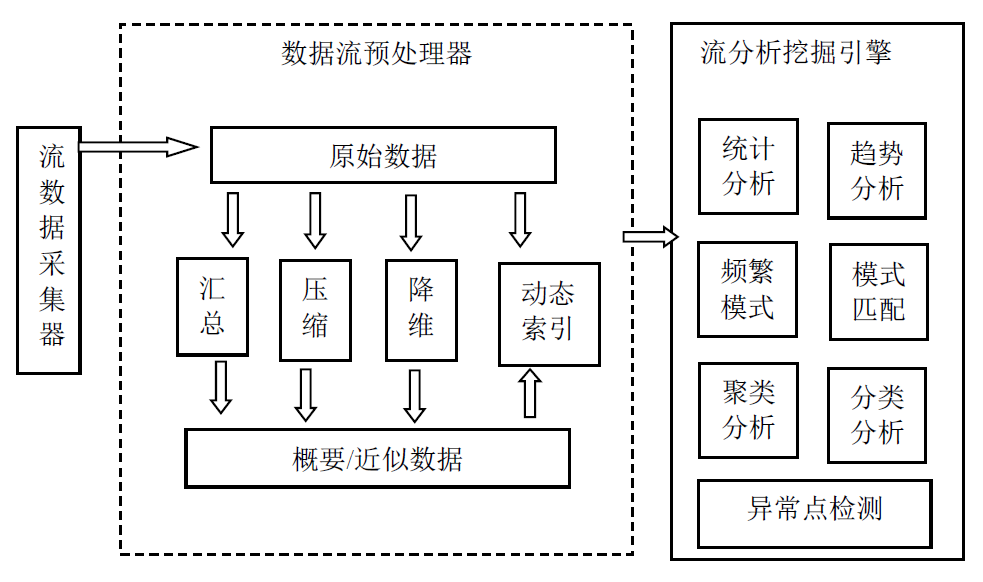
\includegraphics[width=0.75\textwidth]{figures/figure1x1}
	\caption{流式数据分析与挖掘系统模型}\label{fig:fig1}
\end{figure}

流式数据是连续的随着时间产生的数据序列,其中的数据可以是关系元组,也可以是数据项。目前在数据流研究领域存在多种数据流模型,分别有时序模型,现金登记模型和十字转门模型\upcite{孙玉芬2007流数据挖掘综述}。假设流式数据$X$的数据项为 ${x}_{1},{x}_{2},{x}_{3}, ..., {x}_{i}, ...$,数据项序列的下标$i$按顺序递增的,每个下标出现且只出现一次,则

\textbf{时序模型}:\ 每个数据项都代表所描述数据的属性值,$X[i] = {x}_{i}$。

\textbf{现金登记模型}:\ 多个数据项增量地描述数据的属性值,令${x}_{i} = \left(j,{I}_{i} \right)$,其中${I}_{i} > 0$,则有${X}_{i}[j] = {X}_{i-1}[j] + {I}_{i}$。

\textbf{十字转门模型}:\ 多个数据项描述数据的属性值,与现金登记模型的区别是现金登记模型的数据的属性值是一直在增大的,而十字转门模型的属性值可以增大,也可以减小。令${x}_{i} = \left(j,{U}_{i} \right)$,其中${U}_{i}$可以为正数,也可以为负数,则有${X}_{i}[j] = {X}_{i-1}[j] + {U}_{i}$。

其中,时序模型在流式数据的分析和挖掘中应用比较广泛。时序数据的数据项是一个关系元组$\left \langle t,s \right \rangle$,其中,$t$为时间戳,$s$为$t$时刻对应数据的属性值。数据流的数据具有时效性,因此数据携带有时间特征,通常为产生时刻的时间戳。流式数据要求对它进行实时性处理,数据项一旦流过就不复存在,不能再次进行访问,流式数据是源源不断产生的,具有潜在的无限体积,因此不能被全部存储下来。这些都是流式数据的特点。

\section{主要研究内容}
本文主要对流式数据的分析和处理进行研究。针对流式数据的特点,研究异常数据检测和数据压缩的常用算法,探讨在流式计算环境下,如何对算法更好地使用和优化加速,提高流式数据的处理效率。

异常数据检测的任务主要是从数据集中有效地检测出异常数据,异常数据是指在数据集中不符合正常行为模式定义的数据模式,也称为离散点。异常数据在数据集中所占比重小,采样困难,但是其中一般存在重要的信息,或者如果不进行检测,会对后续的处理产生重要的甚至灾难性的影响。比如在工业中,机器发生故障,此时通过异常点检测可以及时发现故障机器,减少生产损失。在日常生活中,电信欺诈和信用卡欺诈等行为已经造成了恶劣的社会影响,通过对正常数据生成模型,通过算法检测异常行为,可以有效地避免欺诈行为的发生,保护财产安全。异常数据检测还可以应用在网站维护方面,如果网站的访问量突然大幅度增加,可能原因是网站被黑客攻击或者被爬虫爬取数据等,所以异常数据的检测,在各个方面都具有实际的应用价值,对其进行研究具有重要的意义。目前为止形成了很多较为成熟且实用的方法,例如基于统计的方法、基于距离的方法和基于聚类的方法等。但是,由于时间复杂度和空间复杂度的影响,部分异常数据检测算法多为静态检测方法,适用于维度较低规模较小的数据集的离线检测,而流式数据大多维度高规模大,并且数据是源源不断到来的,数据量不断动态增长,行为模式可能随时间发生变化,所以在流式计算中,许多成熟的静态异常数据检测算法往往会出现检测结果发生偏差的问题,存在精度不高,运行效率低,不再适用等不足。

由大数据的特点可知,数据的数据量巨大,价值密度很低,对数据进行存储,不但需要耗费比较昂贵的存储资源,而且直接存储价值较低的原始数据没有意义。原始数据常常有噪音干扰,将原始数据直接存储后进行分析和挖掘会消耗大量的计算时间和存储空间,而且也会影响算法的准确性和可靠性。对原始数据进行压缩,可以减少数据的存储空间,节省存储资源,减少存储和后续的计算代价,而且数据压缩不计较细节上的差异,用整体数据的一些特征点来刻画整个数据的主要形态,保留这些主体特征,反应了数据的自身特点。数据压缩可以通过控制压缩度来实现不同的精度层次上的搜索和匹配,更能符合大多数领域只关心数据的变化规律或模式的需求。因此,数据压缩是数据预处理环节中重要的一项内容,具有重要的研究意义。在流式计算中,数据流是源源不断持续增长的,在对数据进行压缩时,数据产生的速度很快,如果压缩花费的时间较多,数据的处理不及时,未处理的数据容易拥塞聚集,最后很可能造成数据丢失的严重后果,因此在流式计算中,对压缩算法进行加速有很重要的意义。

本文主要研究流式数据的数据压缩和异常数据检测的时效性问题,来满足流式数据数据规模大,实时性强的特征,以及在线处理的要求。具体来说,针对流式数据的压缩与异常数据检测,完成以下工作:

第一,针对增量LOF算法在流式数据处理中存在的问题,提出了一种改进的增量LOF快速异常数据检测方法,该方法将数据的分布空间进行划分,将数据点映射到对应的网格单元中,可以有效解决流式数据数据量巨大无法在内存中存储计算的问题,而且减少了计算量。在此基础上,将同一网格内的数据点集中到中心一点,对数据点进行基于密度的异常数据检测,这种方法一方面可以减少数据的存储量,另一方面减少了需要进行距离运算的对象,大大减少了计算量,具有很好的时效性和较少的空间消耗。

第二,根据流式数据在线压缩的要求,采用滑动窗口算法与分段多项式拟合算法来对数据进行压缩。针对时序数据的采样时间是否是周期的,分析在多项式拟合中计算多项式系数时所用的最小二乘法的过程,分别采用缓存方法和增量计算的方法,减少计算量,来对数据压缩进行加速。

第三,通过实验,验证了本文针对数据压缩和异常数据检测提出的加速算法的有效性,减少了计算时间,保证了流式数据处理的高实时性。针对基于LOF方法的快速异常检测算法,通过实验对比,验证了本文的算法可以很好地适用于流式计算环境中,并且取得较好的结果,并且处理数据的速度更快,运行内存更小。针对数据压缩的加速   算法,通过实验,验证了本文提出的算法在不同多项式次数和不同误差率的情况下,可以很好地减少运行时间。

\section{章节安排}
本文主要分析异常数据检测和数据压缩在流式环境下的主流算法,探求算法的可行性和效率,基于这些算法提出改进,使计算提高效率,减少计算时间,达到加速效果。然后进行实验分析,保证其在实际中可以应用的可行性。本文的章节安排如下。

第一章,绪论,介绍了研究背景和意义,介绍了大数据的定义与特点,并介绍了大数据的计算模式,分为批量计算和流式计算,介绍了流式数据的特点和流式数据的处理计算模型。

第二章,针对异常数据检测方法和数据压缩方法,分别阐述了其应用背景,方法概述,和相关实现方法。这部分主要介绍异常数据检测方法和数据压缩方法的研究现状和主要使用算法。总结了异常数据检测的相关研究成果,介绍了主流的异常数据检测算法,包括基于统计的、基于聚类的、基于距离的和基于密度的方法。并且介绍了经典的算法,如iForest算法,LOF算法等等。总结了经典的数据压缩的方法,包括奇异值分解法、分段线性法、符号表示法和频域法,分析了各种方法优缺点及应用范围。以及很多方法都是应用在静态数据集中的,在流式数据的计算中,该如何改进使用这些方法。

第三章,介绍了异常数据检测方法的LOF方法和适用于流式数据的增量LOF算法,并且基于这两种方法,提出了一种新方法,该方法相比于增量的LOF方法,减少了存储量和计算量,更适合流式数据。

第四章,介绍了分段多项式压缩的方法,首先分析了在静态数据集上如何进行加速计算,然后针对流式数据给出了滑动窗口算法与分段多项式相结合的压缩算法,最后通过分析其压缩过程,对于不同的数据类型,给出了不同的加速计算方法。

第五章,实验章节,主要分为异常数据检测的对比实验和压缩算法的对比实验。异常数据检测算法主要与增量的LOF算法进行对比,压缩算法与原计算方法进行不同多项式次数的时间对比与不同分段方法的时间对比。

最后对论文的主要研究内容进行了总结。
\chapter{相关工作}
\label{chap:intro}

为了保证软件的可靠性和稳定性,在大量研究人员长期不懈地努力下,出现了很多针对软件缺陷的检测方法。这些方法可以在软件开发周期的不同阶段介入,检测的效率和效果也大不相同,最终涌现出了一批相对成熟的代码缺陷检测方法和工具。另一方面,随着软件数量的日益庞大,以及数据挖掘技术在各个研究领域的广泛应用,利用机器学习的方式来解决软件安全问题也逐渐成为了研究热点。

\section{程序静态分析技术}

静态分析技术即是在不运行程序,不依赖程序输入的情况下对程序代码进行分析的一项技术。这种技术有助于开发人员对代码结构的理解,同时也能检测潜在的安全缺陷(如SQL注入),运行时错误(如空指针引用缺陷)以及部分代码逻辑错误。它一般需要配合利用自动化工具执行分析。采用的技术有数据流分析,机器学习,语义精简等。可检测死锁,空指针,资源泄露,缓存区溢出,安全漏洞,竞态条件等软件缺陷,具有快速,准确,伸缩性强等特点。能够在代码开发阶段找到并修复多种问题,从而节省大量人力成本和时间。下面对部分静态分析方法涉及的相关技术进行简要的介绍。

符号执行\cite{king1976symbolic}是静态分析中较常用到的一种技术,它可以利用抽象符号描述程序执行过程中的变量值。这种方法可以很好地模拟程序的运行过程。相对于传统方法无法确定程序真实执行下各变量值的情况,此方法在对程序进行路径敏感分析时十分有效。不过因为符号执行方法会追踪程序中所有变量的所有取值空间,所以在应用于大规模代码进行分析时,可能会导致分析的可能路径数量迅速增多,因此在应用该方法的时候,往往会采取优化路径数量的方法即选择部分可能性最高的路径进行分析,这样虽然可以避免状态爆炸的产生,但是也难免会导致分析精度的下降。

PREfix\cite{bush2000static}是一种针对C语言的静态分析工具,它采用了符号执行的方法。该工具可以对程序每个可能的执行过程进行抽象建模,静态地模拟程序的多个可能执行路径,同时利用约束求解对程序分析过程中出现的约束集合进行检查。此工具能够做到路径敏感的缺陷检查,但是由于符号执行方法的特性,为了避免状态爆炸的情况出现,它只能选取部分路径进行分析,这就导致了分析精度的不理想。

模型检查\cite{jhala2009software}也是一种常见的静态分析技术,通常的做法是构建有限状态机或者有向图等抽象模型,再对构造出的模型进行遍历来检验待检测系统的部分性质。SLAM\cite{ball2001automatically}是一种具有代表性的基于模型检查的静态分析工具。它可以从待检测代码中抽象出一个布尔程序并加以验证。在得到的错误报告中逐个检查,找出所有误报,进而根据这些误报对抽象的布尔程序进行调优,经过不断迭代,最终可以取得很好的效果。

同样是应用于程序验证的技术,不同于模型检查,定理证明\cite{tiwari2007logical}是基于语义的程序分析方法。但是由于采用了消解原理的定理证明器,而这种方法对整数域和有理数域相关的运算不是很好处理,所以应用在程序分析领域显得不是特别合适。基于这种问题,研究人员通常会选择各种判定过程来确定公式是否是定理。ESC\cite{flanagan2013pldi}就是一个采用了定理证明技术的半自动化工具,它在分析程序的过程中需要外界指定所涉及的类不变量,过程不变量以及循环不变量。

除了上面提到的3种技术,抽象解释\cite{cousot1977abstract}的应用更加广泛,它是数据流分析的理论基础。1977年P.Cousot和R.Cousot
共同提出了抽象解释的理论,应用该理论分析程序时就不需要拘泥于程序最底层的具体细节上可以在更高的角度上去观察和思考。传统解释器可以知道程序中每个变量具体的值从而得到具体值域,而抽象解释不同与传统解释的地方就是可以得到一个更高阶的抽象值域。如果将一个传统解释器迁移到抽象解释器,几乎等同于构造一个函数把具体值域映射到抽象值域。如图\ref{fig:figure2-1}所示,我们可以将无限的整数具体值域抽象成正,负,零三个抽象值域,这个过程只需要实现一个抽象函数$\alpha$即可完成。
 \begin{figure}
	\centering
	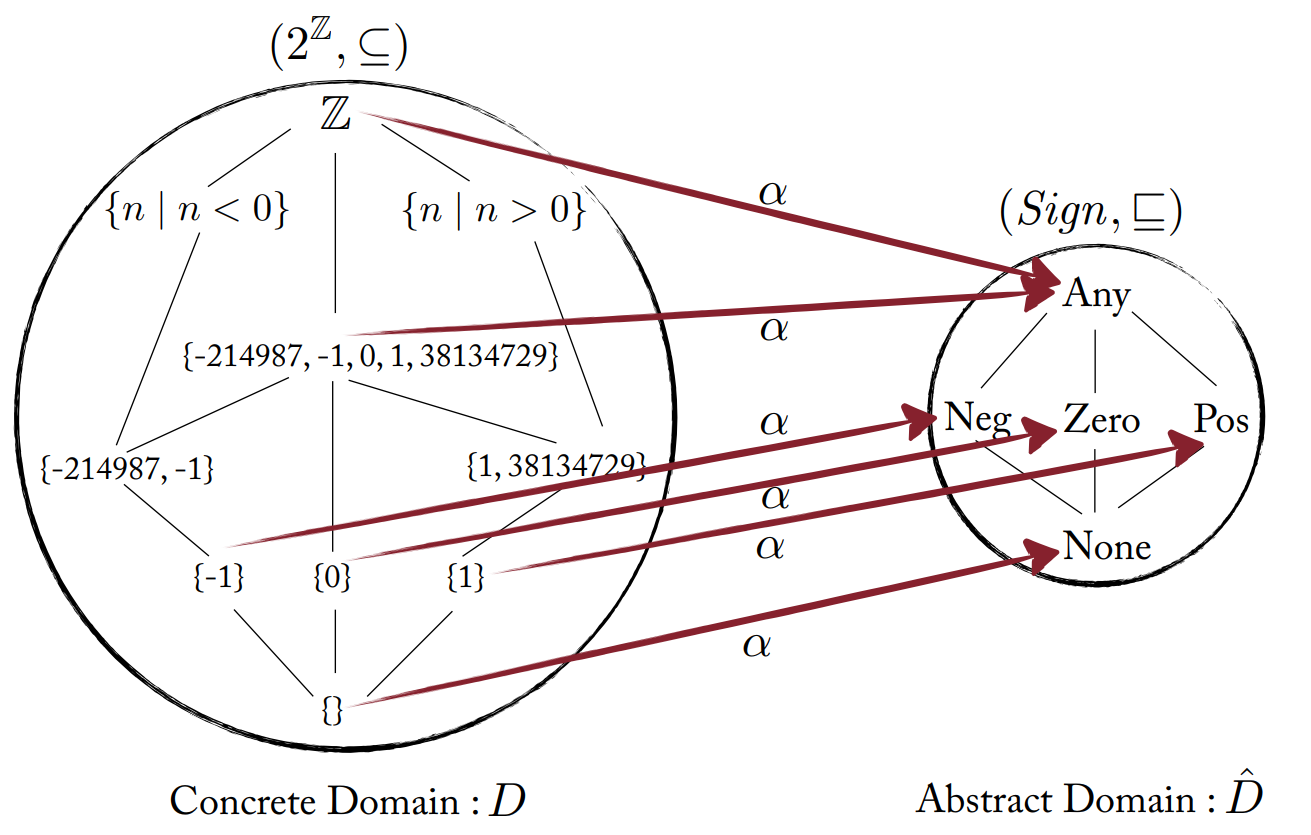
\includegraphics[width=0.70\textwidth]{figures/AbstractInterpretation2-1}
	\caption{将整数空间的具体值域映射到抽象值域}\label{fig:figure2-1}
\end{figure}

抽象解释理论实际上是从代码中抽象出一些能够刻画我们想要分析的问题所需要的特征,本质上还是为了提升分析的效率而损失部分分析精度的方法。但是如果应用得当,还是可以获得很大的收益,现在几乎所有的数据流分析方法都应用了该理论。

总的来说,静态分析技术在不运行代码的情况下进行分析有效避免了程序运行环境的苛刻要求,可以针对程序的规模采取灵活的分析方法,从而具备了较早发现缺陷,较低的分析成本,较高的覆盖率和自动化程序等优点。但是由于往往需要对分析精度进行部分舍弃,导致了分析结果的漏报率和误报率都无法达到特别理想的水平。

\section{静态分析技术在空指针引用缺陷检测的应用}
针对空指针引用缺陷,研究人员已经利用静态分析技术做出了很多实践并取得了一定成果。

研究人员利用静态分析技术在Java空指针引用缺陷上进行了大量的工作,产生了很多检测空指针引用的工具和技术,这些技术可粗略的分为指针引用验证\cite{madhavan2011null}和空指针引用\cite{xie2007saturn}缺陷检测两大类。前者侧重于如何验证程序中的指针是否为空。后者侧重于如何尽可能多的发现程序中的空指针引用。指针引用验证技术是基于需求驱动的思想\cite{wang2015},一般是首先识别出指针,再沿着控制流后向的验证指针是否为空。空指针引用缺陷检测一般是在进行数据流分析\cite{wangxu2015}、指针分析的基础上,根据一些规则基于控制流前向的检测。两者通常都需要进行数据流分析与指针分析。

Salsa\cite{loginov2008verifying}是一个致力于验证Java代码中指针引用安全性验证的工具,通过定制的数据表示形式进行前向数据流分析,通过对传播深度和数据流传播路径数量的简单限制来获得方法的可扩展性,同时依赖预先进行的必然别名分析来提高方法间数据流分析的准确性。由于一些空指针的引用需要经过多层方法调用链才有可能触发,这种验证方式会产生很多漏报的同时,效率也不理想。数据流分析技术具有十分灵活的特点,为了提高效率,Ravichandhran Madhavan\cite{madhavan2011null}等提出了一种过近似的最弱前置条件分析方法以验证Java程序中指针的安全性,该方法通过需求驱动的前向数据流分析大幅提升了单个引用的分析效率,该方法试图找到程序入口处可能满足被分析程序点的引用不安全的条件,如果存在这样的条件,则可以判定该引用不安全。此方法的数据流事实为有限的谓词集合,通过有选择地限制谓词集合的大小以及传播路径的数量,该方法可以做到低延迟的流敏感,上下文敏感的sound分析,利用Wala\cite{wala}程序分析框架,可以取得较好的验证引用安全的效果,但是过于追求针对单个引用的需求驱动分析,在对大规模代码中的引用进行批量分析时性能欠佳。

空指针检测相比于指针安全性验证更加具有实用性,而误报率和漏报率是检验工具实用性的重要指标,空指针检测工具大多不追求完美的正确率,而将较低的误报率和较高的召回率作为最重要的目标。

检测工具Xylem\cite{nanda2009accurate}从每一个指针引用出发,进行基于需求驱动的后向数据流分析,并将谓词作为数据流事实,目标是能够高效的检测出最重要的空指针引用,在进行分析时采取的是不完全可靠的分析方法,检测结果存在较多漏报。

北京邮电大学的杨睿\cite{yangrui2012}提出一种Java中空指针引用故障的静态检测方法,将空指针引用问题抽象为一类故障模型,并以故障模式状态机来形式化描述此类故障模型,然后根据故障状态机的创建条件及待检测代码的语义信息确定是否创建该类型的状态机,并将创建的状态机示例置于控制流图入口,根据数据流分析的结果对故障状态进行迭代以检测空指针引用问题。

中国矿业大学的姜淑娟\cite{jiang2017}提出一种空指针异常自动定位方法,该方法结合程序的静态分析技术,利用程序运行时的堆栈信息指导程序切片,然后对得到的切片进行空指针分析及别名分析,得出引发空指针异常的可疑语句集合,最终给出错误定位报告。

总体来看,以上这些分析方法都有各自的优缺点,但是目前无法找到一种完美的静态检测方法可以兼顾缺陷检测的误报率和漏报率。这也正是静态代码分析的短板,不仅是将复杂的缺陷解释出来很困难,对于结果的高误报率,往往显得无能为力。

\section{代码缺陷检测工具介绍}
对于空指针引用缺陷,工业界已经产生了很多优秀的检测工具,这些工具具有不同的实现原理,对空指针引用缺陷的检测结果也不尽相同。

FindBugs\cite{hovemeyer2005evaluating}\cite{hovemeyer2007finding}是一个开源的针对Java代码的缺陷静态检测工具,通过分析class文件,在字节码层级进行简单的前向数据流分析,对程序中的每一个引用的是否为null值的不同情况,给定相应的标识从而在触发可能的空指针调用时给出不同的告警等级。对于指针引用FindBugs总结出了一些经验规则,对不可达路径、控制流汇合、指针赋值语句、断言等特定情况定制了专用的检测规则,在进行过程间分析时,其主要依赖特定故障模式以及用户编码时给出的注解来推断空指针是否可能发生,所以它只能在特定场景下检测出空指针引用缺陷。

Jlint同样是一个开源静态代码检测工具,它通过执行数据流分析和构建锁图来查找缺陷,语义矛盾和同步问题。Jlint有两个独立的程序来执行语法和语义验证。通过使用手写扫描器和简单的自顶向下解析器,Jlint能够检测到一些代码缺陷,例如可疑地使用操作符优先级,没有切换代码中断,对构造体错误的假设等。同时,Jlint执行本地和全局数据流分析,计算局部变量的可能值并捕获冗余和可疑计算。通过执行全局方法调用分析,Jlint能够检测具有可能为“null”的形参的方法的调用,并且在没有验证“null”的方法中使用该参数。 Jlint还为类依赖项构建了锁依赖关系图,并使用该图来检测在多线程程序执行期间可能导致死锁的情况。除了死锁之外,当不同的线程可以同时访问相同的变量时,Jlint能够检测到可能的竞争条件问题。Jlint最大的特点就是检测的效率很高,但是由于使用的数据流分析十分有限,因此误报率也较高。

Infer是Facebook的开发团队在代码提交内部评审时,用来执行增量分析的一款静态分析工具,在代码提交到代码库或者部署到用户的设备之前找出缺陷。由OCaml语言编写的Infer目前能检测出空指针访问、资源泄露以及内存泄露,可对C、Java或Objective-C代码进行检测。Facebook使用Infer自动验证iOS和安卓上的移动应用的代码,bug报告的正确率达80\%。Infer通过捕获编译命令,把要被编译的文件转换为可用于分析潜在错误的中间语言格式。整个过程是增量进行的,意味着通常只有那些有修改过并提交编译的文件才会被Infer分析。Infer还集成了大量的构建或编译工具,包括Gradle、Maven、Buck、Xcodebuild、clang、make和javac。此外,Infer根植于两大基本理论之上,其一是霍尔逻辑,一种用于推理计算机程序正确性的形式系统,另一个是抽象解释,该理论用于测度程序语义的逼近结果,此外还涉及其它一些研究成果,例如Separation Logic和Bi-abduction。

Fortify SCA是一款应用广泛的商业工具,由知名的惠普公司出品 ,是一个白盒的、静态的软件源代码安全检测工具。它通过内部的五种主要分析引擎:语义、结构、控制流、数据流、配置流等对应用程序的源码进行静态分析,在分析的同时与该工具特有的软件安全漏洞规则集进行全面地查找、匹配,进而找出源代码中存在的各种缺陷和漏洞,并整理和产出缺陷报告。Fortify应用十分广泛,在世界范围内被大量公司用作内部源代码的质量安全检测工具。

Coverity是美国Coverity公司提供的可配置的用于检测软件缺陷和安全隐患的静态源代码分析解决方案,该工具基于布尔可满足验证技术应用于源代码分析引擎,分析引擎利用其专利的软件DNA图谱技术和meta-compilation技术,综合分析源代码、编译构建系统和操作系统等可能使软件产生的缺陷。Coverity是第一个能够快速、准确分析当今的大规模、高复杂度代码的工具,它解决了影响源代码分析有效性的很多关键问题,如编译兼容性,构建集成,高误报率,有效的错误根源分析等。

\section{深度学习技术在软件安全领域的应用}
深度学习是人工神经网络中一种多层级学习框架,试图通过构建深层网络模拟人脑感知抽象概念的能力。近年来,深度学习凭借着强大的特征学习能力,问题表达能力,数据容纳能力,掀起了又一次机器学习的浪潮,并在计算机视觉,语音处理,自然语言处理等众多领域取得了巨大进展,受到从学术界到工业界的广泛关注。现在,深度学习技术也开始渗透进软件工程的多个领域。

由于代码作为输入数据的特殊性以及复杂性,深度学习在软件安全方面常见的应用方法有两种。一种是以自然语言处理的思想来挖掘代码里的潜在信息;一种是将代码抽象为控制流图,以控制流图作为输入,压缩控制流图为向量之后进行分类回归运算。

Martin White\cite{white2016deep}等人提出了一种自然语言处理算法检测代码克隆的方法,该方法使用了两个RNN(递归神经网络)模型。先运用语法分析对代码进行预处理,然后用第一个RNN网络得到中间向量,再对代码进行词法分析得到代码的抽象语法树,将中间变量和语法树作为第二个RNN网络的输入,得到最终的检测结果。这种方法考虑到了代码文本上的相似性,忽视了代码结构上的相似性。

Hanjun Dai\cite{dai2016discriminative}提出了一种基于神经网络的图特征抽取的算法,能够根据不同的分类标准将代码控制流图压缩为多维的向量。Xiaojun Xu\cite{DBLP:journals/corr/abs-1708-06525}改进了该网络,通过将两段代码的控制流图成对的进行训练,从而检测两个二进制代码的相似度。通过该网络可以预测待测代码与已知缺陷代码的相似度,从而判断该代码是否为缺陷代码,为神经网络在检测代码缺陷方面的应用提供了新的思路。

\section{本章小结}
本章首先介绍了静态分析涉及的相关技术背景,然后以空指针引用的检测为例,介绍了国内外研究人员利用静态分析技术在空指针引用缺陷检测方面的进展,随后对一些业界成熟的静态代码缺陷检测工具,如Findbugs,Jlint,Infer,Fortify等进行了简要的介绍,最后对当下热门的深度学习技术在软件安全领域的应用进行了讨论。
\chapter{总体架构}
本论文的目标是引入深度学习的方法针依据不同工具对代码的检测能力对大量缺陷代码进行分类,在使用多种检测工具对同一份代码进行检测时,可以有效得知这些工具针对这份代码的检测能力,然后利用这些工具的检测报告给出更精准的评判,从而提升检测精度。
\section{设计背景}
随着软件规模的增大,缺陷检测的难度和所需要的代价都越来越大,就Java语言的空指针引用异常的检测来说,目前业界存在着很多工具。如Findbugs,Jlint,Infer,Fortify等。他们在检测缺陷时使用了模式匹配,数据流分析,类型系统,模型检查等技术,由于不同的技术出于对检测精度和效率的权衡,他们所产出的检测报告往往各不相同,并且几乎都包含了大量的误报和漏报,开发人员在面对这样复杂的报告时,很难判断某条报告的准确性。NickRutar[A comparison of Bug Finding Tools for Java]等人针对五种Java语言的缺陷检测工具做了比较,发现没有任何一个单一的工具是完美的,此外,不同工具所产出的报告之间也有不小的差异。

基于这种情况,可以设想将多种工具的报告汇总到一起进行交叉验证,如果多个工具同时给出了同一个位置出现同一种缺陷的报告,我们有理由相信这个缺陷是真实可信的。因此,我们基于sonarqube平台开发了插件BIT-Detector,这个插件集成了Findbugs,Jlint,Infer和Fortify的能力,针对同一份待测代码,首先使用4种工具分别检测并给出报告,然后过滤出空指针引用缺陷,最后将4份报告的内容格式统一化从而进行比对,将不同工具同时检出的空指针引用缺陷作为BIT-Detector的输出,这样的结果理论上可以达到很高的准确率。

由于难以找到合适的空指针引用缺陷数据集,为了对这些工具进行合理的评测,本文采用一种创新的方式构建了一批可信的测试用例,这些用例的构造方法会在后面的章节详细说明。利用构建出来的7429个测试用例,我们针对上文提到的四种工具以及BIT-Detector进行了测试。图\ref{fig:figure3-1}反映了各个工具检出的空指针引用缺陷的重叠情况,表\ref{tab:table3-1}给出了不同工具检测的精度信息,同时还给出了BIT-Detector的数据。通过对比不难发现,各个工具的检测结果确实有较大差异,即使我们使用检测准确度最高的Findbugs,也会面临超过三分之一的误报,这些误报掺杂在检测报告中会给开发人员的缺陷修复带来很多困扰,可能很多时间和精力都会被浪费在验证缺陷的真实性上面。而保证报告的准确性应该是对检测工具的基本要求,即使不谈准确率,过多的漏报也会让人沮丧。显然,目前被广泛使用的各种检测工具还有很大的提升空间。

在检测过程中,我们也注意到选取所有工具共同检测缺陷作为输出结果的BIT-Detector在检测结果的准确率方面有着突出表现,相对于表现最好的Findbugs和Fortify,BIT-Detector有着22\%的准确率提升,而相对于准确率较低的Jlint而言,BIT-Detector的准确率提升则是成倍的增加。即使召回率的表现不尽人意,但是如果我们不将除了四种工具同时检测的缺陷排除在外,而是将四种工具的检测结果按照优先级排序,召回率在某种程度上来讲反而是提升的,如果按照这种方式处理检测报告,此时BIT-Detector的检测结果将自然地排在最前面,但是对其他结果的排序就成了一个棘手的问题,假如我们有四种工具,分别记为$T_{a}$,$T_{b}$,$T_{c}$,$T_{d}$。如果工具$T$在被测代码的$L$位置成功检出了某个缺陷$D$,则记为$E(T,L,D)=1$,反之则记为$E(T,L,D)=-1$。给定位置$L_{i}$,存在如下这种情况

\begin{equation}  
	\left\{  
	\begin{array}{lr}  
	E(T_{a},L_{i},D)=1, &  \\  
	E(T_{b},L_{i},D)=1, &  \\  
	E(T_{c},L_{i},D)=-1, &  \\  
	E(T_{d},L_{i},D)=-1, &  \\  
	\end{array}  
	\right.  
\end{equation} 

在这种情况下,开发人员很难判断位置$L_i$处是否存在缺陷$D$,如果我们知道工具



\begin{figure}
	\centering
	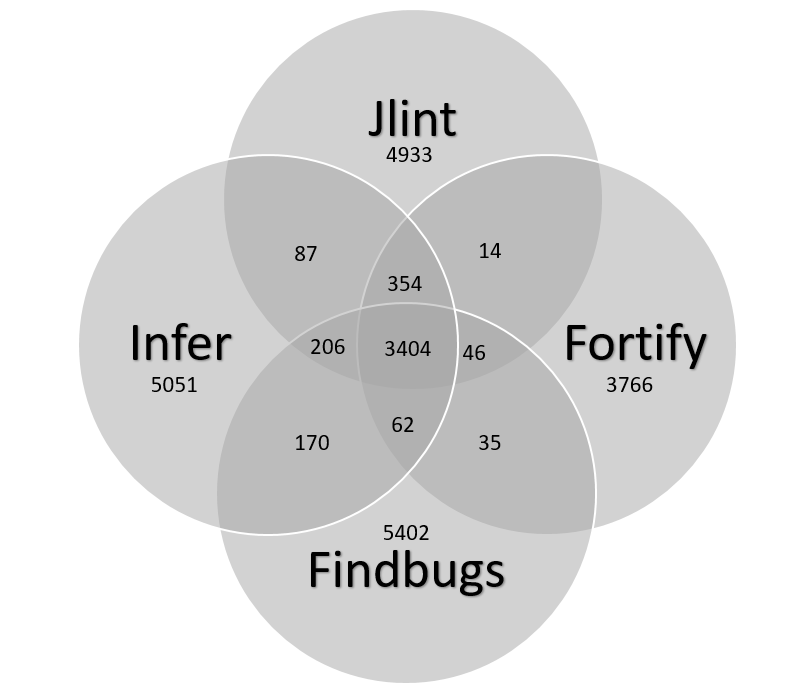
\includegraphics[width=0.70\textwidth]{figures/vnfigure3-1}
	\caption{4种工具在7429个测试用例上的检测结果}\label{fig:figure3-1}
\end{figure}

\begin{table}
	\centering
	\caption{四种工具和BIT-Detector的测试结果对比} \label{tab:table3-1}
	\begin{tabular*}{0.9\textwidth}{@{\extracolsep{\fill}}ccccc}
		\toprule
		测试工具	&正报	&误报	&准确率	&召回率 \\
		\midrule
		Findbugs	&5402	&3169	&63\%	&72\% \\
		Jlint	&4933	&9137	&35\%	&66\% \\
		Infer	&5051	&3578	&58\%	&68\% \\
		Fortify	&3766	&2211	&63\%	&50\% \\
		BIT-Detector	&3404	&576	&85\%	&45\% \\
		\bottomrule
	\end{tabular*}
\end{table}
\section{设计思路}
\section{整体架构}
\section{组织结构}
\section{本章小结}
\chapter{数据集的构建和预处理}

上一章节提到模型的构建需要大量的测试用例,由于合适开源用例的稀缺,合理利用现有无缺陷代码来生成空指针引用缺陷是一种可行的方式。为了便于后续的处理工作,测试用例的选择应该从多维度慎重考虑。然后,为了模型训练的顺利进行,还需要对这些数据进行预处理,构建出正确的控制流图,提取出合适的代码特征。这些工作都是神经网络模型训练所依赖的重要基础。

\section{数据集构建}
\subsection{数据来源}
如果采取从正常代码中构造空指针引用缺陷的方式,首先面对的问题就是选择构建用例的合适的代码资料。为了便于后期处理,用例应该包含程序入口,具备语义完整,结构多样化,代码规范简洁等特点,只要程序包含常见的语法结构和调用关系,程序规模不应过大,恰好包含空指针引用缺陷产生的上下文最佳。依据这些条件,本文选择了部分开源代码数据集作为构建空指针引用缺陷的原始资料,如图\ref{fig:figure4-1}所示。

\begin{figure}
	\centering
	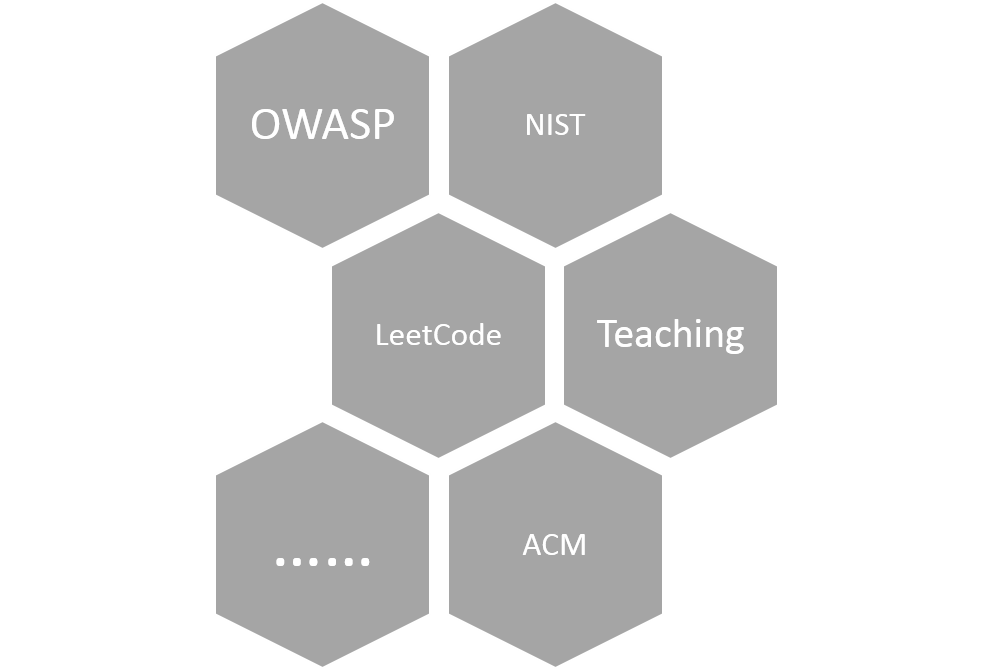
\includegraphics[width=0.70\textwidth]{figures/resource4-1}
	\caption{测试用例来源}\label{fig:figure4-1}
\end{figure}

其中,OWASP和NIST分别为代码缺陷检测相关领域的项目。从这些项目下可以获得部分标准的空指针引用缺陷用例,同时也可以得到很多具备其他缺陷的测试用例。由于这些用例的代码编写较为规范并经过了合理分类,还往往包含说明文档等辅助理解代码的信息,大多都可以用来生成空指针引用缺陷。除此之外,LeetCode和ACM作为编程竞赛性质的项目下也包含大量可以利用的代码,这些代码根据题目的难易级别具备着不同的复杂程度,包含了多样的代码结构,同时,这些代码的规模往往不大,是作为空指针引用缺陷用例构造的良好资源。另外,一些供教学使用的代码也是十分合适的空指针缺陷构造来源。作为补充,本文还添加了部分人工编写的测试用例。

\subsection{缺陷用例构造}
在取得构造缺陷用例的原始代码后,需要对这些代码进行检查,确保代码有正确的程序入口,并且可以正确执行。对于OWASP和NIST项目下的代码,很多用例缺乏Main方法的入口,这会导致后续控制流图提取的困难,这时需要在源代码层级加入合适Main方法,调用合适的方法驱动程序的执行。此外,对于ACM和LeetCode项目下的代码资源,虽然所有用例都包含正确的程序入口,但是往往需要正确的标准输入流数据程序才能正确执行。获得这些用例的输入数据并不困难,只需要按照相应题目下的输入输出样例给予输入数据即可驱动程序执行,这些数据的获取可以通过爬虫程序取得,自动化输入数据则可以通过重定向程序的输入流来完成。

空指针引用缺陷的产生必然需要一个产生null值的缺陷源。在程序的某个位置,变量被赋值为null,随后沿着控制流图向前传播,在遇到对该变量的解引用时便会触发空指针引用异常。这个变量便是缺陷源,只要在程序中的合适位置构造缺陷源,则有一定的可能会在程序的下文中触发空指针引用缺陷。当原始代码的可用性得到确认后,需要对程序进行语法分析,寻找合适的空指针产生点并构造缺陷源。

对Java文件进行语法分析可以使用Eclipse JDT下的AST来完成,该工具可以在Eclipse环境下获得。利用它能够对Java文件进行解析,生成相应的抽象语法树,并且能够任意修改Java代码的语法结构。在AST中,Java代码的每一个语法结构都有对应的AST结点表示,这些结点具有完整的层次关系,可以表示整个程序对象到具体方法的某个具体变量。如图\ref{fig:figure4-2}所示,一个for循环的代码片段按照Eclipse AST的标准解析出抽象语法树,表\ref{tab:table4-1}表示部分结点在AST树中对应的名称。

\begin{figure}
	\centering
	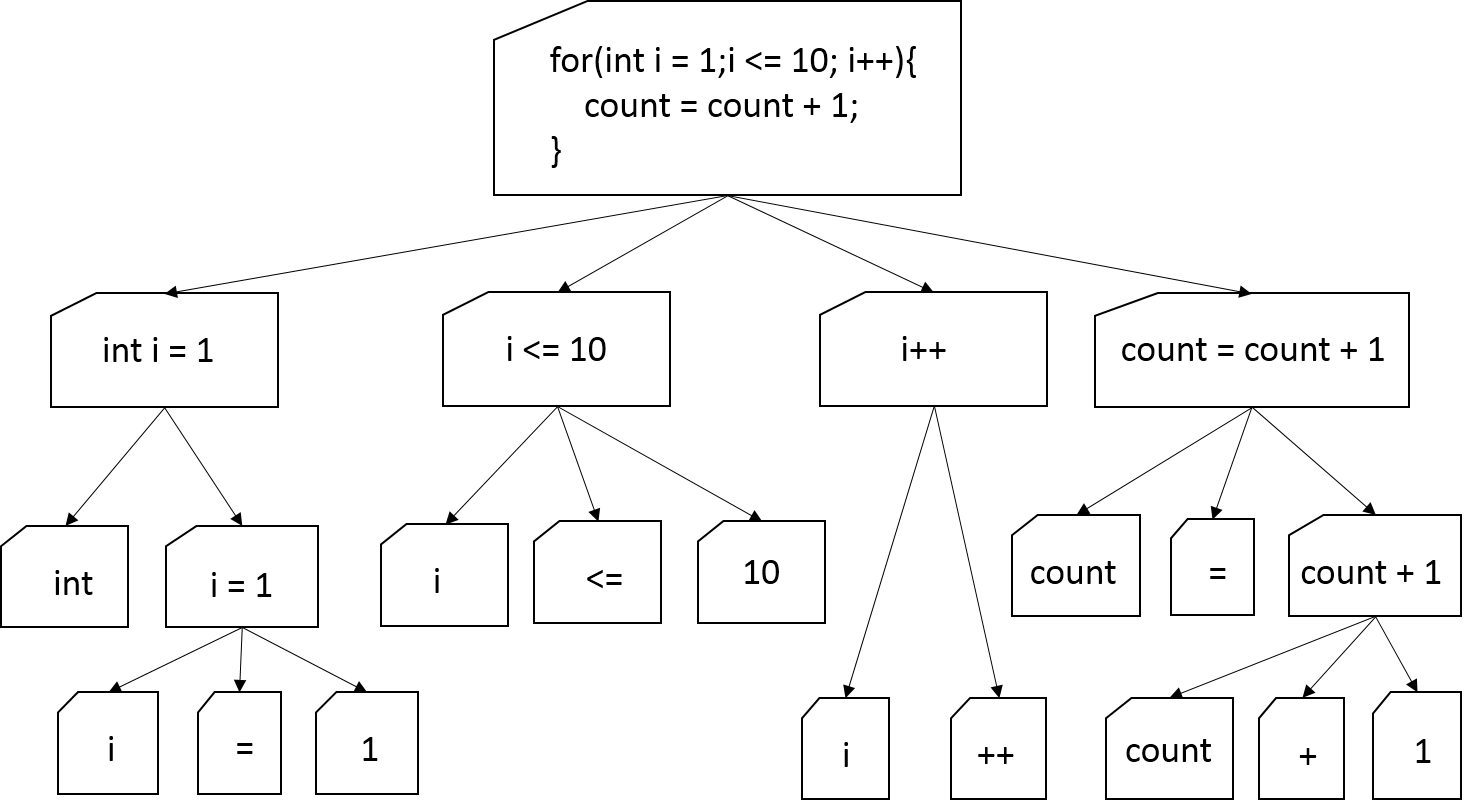
\includegraphics[width=0.70\textwidth]{figures/ast4-2}
	\caption{抽象语法树示例}\label{fig:figure4-2}
\end{figure}

\begin{table}
	\centering
	\caption{AST中的结点信息} \label{tab:table4-1}
	\begin{tabular*}{0.9\textwidth}{@{\extracolsep{\fill}}ccc}
		\toprule
		子节点	&子节点名	&依附于父结点的角色 \\
		\midrule
		int i = 1	&VariableDeclarationExpression	&INITIALIZERS \\
		i <= 10	&InfixExpression	&EXPRESSION \\
		i++	&PostExpression	&UPDATERS \\
		{ count = count + 1 }	&Block	&BODY \\
		\bottomrule
	\end{tabular*}
\end{table}

在生成用例的抽象语法树后,只要找到合适的点位,就可以通过修改相应的操作数为null来构造空指针引用缺陷源。通常这些点位都和赋值表达式有关,但是在过程间调用的上下文中,方法的参数和返回值都可以是合适的构造点位。可以利用的修改位置如下:

(1)类的属性成员。

(2)方法内的局部变量。

(3)方法的参数。

(4)方法的返回值。

其中(1)中的属性成员包含被初始化的非null的普通属性和静态属性。(1)和(2)需要找到相关的赋值表达式,通过修改右操作数为null来生成空指针引用缺陷源。(3)需要判断被调用方法的参数列表中属性的类型,将引用类型的实参修改为null即可。(4)需要判断该方法的返回值类型,只有返回值为引用类型才可以修改。

图\ref{fig:figure4-3}为空指针引用缺陷用例构建的流程图,在抽象语法树的基础上进行修改获得缺陷源后,需要对程序进行编译并执行才能确定能否真正构建出空指针引用缺陷用例。如果没有通过编译或者运行后没有发生空指针引用缺陷,则用例构造失败,需要重新寻找新的构建点位。重复此步骤直到成功产生空指针引用缺陷。最后,成功构建的缺陷用例需要在代码中添加代码信息的注解表明该缺陷的缺陷源和发生空指针解引用的位置。运用注解的方式是为了后续代码信息抽取的工作顺利进行,因为Java程序可以很方便地抽取代码的注解信息,而这些自定义注解不会对代码的实际语义产生影响。记录空指针解引用的位置是为了验证工具检测的结果,加上缺陷源的位置可以很方便的确定该空指针引用缺陷发生的上下文范围,确定分析域。这些注解信息需要放置在测试用例的Main方法所在类中,方便代码信息抽取时统一处理。如果缺陷的产生位置不在Main方法所在类的方法中,就需要在注解信息中表明该缺陷产生位置所在的类。

\begin{figure}
	\centering
	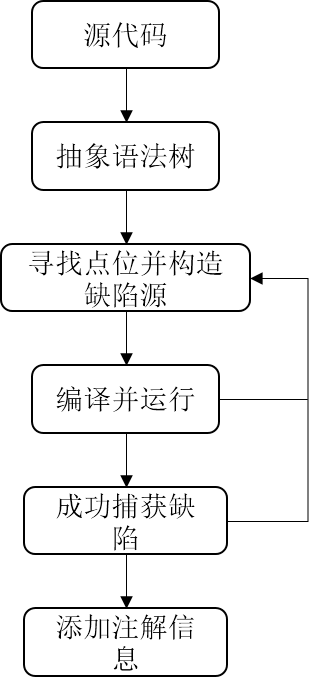
\includegraphics[width=0.25\textwidth]{figures/parse4-3}
	\caption{测试用例构建流程}\label{fig:figure4-3}
\end{figure}

下面的代码片段就展示了一个成功生成的测试用例,在代码的第8行将$sb = new StringBuilder("")$修改为$sb = null$,随后在代码的第11行即对$sb$进行解引用操作,触发空指针引用缺陷。在第一行的注解标注了该缺陷涉及的上下文代码行号及变量名,这表示了分析域的范围。这个例子非常简单,实际上产生的代码在复杂度上各不相同,选用的原始代码往往都具备跨方法和跨文件的调用关系。 

\begin{lstlisting}[language={[AspectJ]Java},numbers=left,keywordstyle=\color{blue!70},commentstyle=\color{red!50!green!50!blue!50},frame=shadowbox, rulesepcolor=\color{red!20!green!20!blue!20}] 
$@Context(start = 8, end = 11, var = “sb")$
public static void main(String[] args) {
      Scanner in = new Scanner(System.in); 
      int k = in.nextInt();
      if(k > 36){
           System.out.println("-1");
      }else{
          StringBuilder sb = null; //source                 
          int mul = k/2;
          while(mul-- > 0){
              sb.append("8"); //npe
          }
          if(k%2 == 1){
              sb.append("4");
          }
          System.out.println(sb.toString());
      }
}
\end{lstlisting}

\section{控制流图提取}
控制流图(Control Flow Graph,CFG)是一个程序或者过程的抽象表现,代表了程序执行过程中所有可能经历的路径信息,能准确刻画程序的结构信息。空指针引用缺陷测试用例生成完毕后,需要生成程序的控制流图。
\subsection{Soot}
Soot\cite{vallee2010soot}是一种Java字节码优化框架,凭借着对Java语言强大的分析能力,已经被广泛地应用于很多针对Java语言的分析优化项目。Soot框架最大的特点是提供了四种不同的代码中间表示形式:Jimple,Baf,Grimp和Shimple,它们考虑到不同的分析场景,对代码进行了不同程度的抽象表示。同时,Soot还构建了自定义的数据结构来表示待分析的项目,这些自定义类型与Java代码中的层次结构一一对应。如表\ref{tab:table4-2}所示。这种表示方法使得代码的分析过程变得更加简单和灵活,易于理解使用。Soot的工作过程如图\ref{fig:figure4-4}所示。

\begin{table}[hb]
	\centering
	\caption{Soot中表示项目的数据结构} \label{tab:table4-2}
	\begin{tabular*}{0.7\textwidth}{@{\extracolsep{\fill}}cc}
		\toprule
		类名	&描述	 \\
		\midrule
		Scene	&表示整个分析环境\\
		SootClass	&表示一个class	\\
		SootMethod	&表示一个Method	 \\
		SootField	&表示一个类成员属性	\\
		Body	&表示一个方法体 \\
		\bottomrule
	\end{tabular*}
\end{table}

\begin{figure}
	\centering
	
\includegraphics[width=0.50\textwidth]{figures/Soot4-4}
	\caption{Soot工作流程}\label{fig:figure4-4}
\end{figure}

Jimple是Soot框架中最主要的代码中间表示形式,采用了典型的基于三地址的语句表达形式,它可以由Java源代码或者Java字节码转换得到。其中,通过字节码的转换通过为隐式的堆栈变量引入新的局部变量以及清除jsr指令来完成。在代码转换的过程中,Jimple中的局部变量会被加上被推断出来的类型信息,同时部分没有用到的局部变量也会在优化阶段被清除掉从而不会出现在Jimple代码中。最重要的是代码中所有的表达式都会经过线性化的处理,最终Jimple将由若干三地址表达式组成。这些表达式至多包含三个变量或者常量信息,这种规则对于执行代码优化是非常方便的。另一方面,Jimple表示形式所包含的语句类型只有15条,相比于Java字节码中多达200多条的指令类型,Jimple的表示形式是足够简洁的,这些精简之后的指令类型也给本文后续的代码特征提取提供了极大的便利。

除了简洁准确的表示形式,利用Soot还可以进行复杂的别名分析和数据流分析。另外,每个待分析方法的方法体,即表\ref{tab:table4-2}中的Body,都包含了一个Units链。Unit是Soot中的一个接口,具体实现则是一个三地址表达式,这些表达式实际上会对应到Jimple中的某个具体语句类型,即Stmt。这些Unit已经包含了互相之间的结构关系,根据这些结构关系可以很方便地生成方法内的控制流图。同时,对于包含调用方法语句类型的Unit,通过Soot提供的API还可以很方便的得知该调用的对象方法,这对后面过程间调用图的构建也非常重要。

\subsection{全局控制流图构建}
上一节介绍了Soot,利用它可以构建出方法内的控制流图和过程间的调用图,进而得到全局控制流图。

方法内的控制流图可以从以Jimple表示的方法体中包含的Units链得到。通过遍历Units链中的Unit元素,可以得到它们的前驱和后继结点,这些信息实际上就表示了该方法的控制流图,不过它的结点是一个Jimple表示的Stmt,在Jimple中表示了一种语句类型。如下面的Jimple代码片段所示,不同的语句对应着Jimple中不同的Stmt类型,这些类型有15种之多,是Jimple能够表示的最基本的语法单位。
\begin{lstlisting}[language={[AspectJ]Java},numbers=left,keywordstyle=\color{blue!70},commentstyle=\color{red!50!green!50!blue!50},frame=shadowbox, rulesepcolor=\color{red!20!green!20!blue!20}] 
public int foo(java.lang.String){//locals
    r0 := @this; // IdentityStmt
    r1 := @parameter0;
    if r1 != null goto label0; // IfStmt
    $\$$i0 = r1.length(); // AssignStmt
    r1.toUpperCase(); // InvokeStmt
    return $\$$i0; // ReturnStmt
label0: // createdbyPrinter
    return2;
}
\end{lstlisting}
从该代码块中可以抽取出foo方法包含的Units链,进而得到其结构信息,如图\ref{fig:figure4-5}所示,结点的序号为代码块中语句对应的行号。从图中任意一个结点都可以找到其相邻的前驱和后继结点,这种关系不是静态代码顺序的关系,其考虑了代码执行逻辑的语序。

\begin{figure}
	\centering
	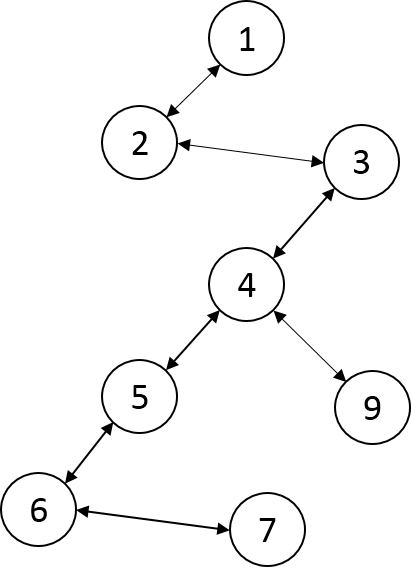
\includegraphics[width=0.25\textwidth]{figures/Units4-5}
	\caption{示例代码的Units关系图}\label{fig:figure4-5}
\end{figure}

过程间调用图的构建需要依赖方法体内的方法调用语句,如上文代码块中的第6行语句,该Stmt的类型为InvokeStmt。实际上InvokeStmt是一个接口,在Jimple包含的Stmt中,实现InvokeStmt接口的类有五种,它们表示五种调用方法的类型:

(1)invokestatic:调用静态方法。

(2)invokespecial:调用实例的私有方法、父类方法或构造器方法。

(3)invokevirtual:调用实例中的虚方法。

(4)invokeinterface:调用接口方法。

(5)invokedynamic:调用动态方法。

其中,前四种调用方式可以由静态分析得到,而invokedynamic调用方式所调用的目标必须在运行时才能动态确定,所以本文只需关注前面四种调用方式,通过对调用目标的解析建立方法之间的调用关系,从而构建出完整的过程间调用图。

这里定义过程间调用图为G,G包含两个数据集合$Caller(U,S_m)$和$Callee(M,S_u)$,前者表示Unit结点与其调用的Method集合的映射关系,后者表示Method与调用它的Unit结点集合的映射关系。由于Unit和Method在Soot分析环境中具有唯一性,并且Unit和Method还包含了其结构的上下文关系信息,即利用Unit可以得到其所属的Method信息,甚至Class信息,所以不需要构建Method与Method之间的调用关系。利用这两个数据集合可以方便地找出某个Unit调用的Method集合$S_m$以及调用Method的Unit集合$S_u$。在Soot开始加载待分析工程时,会将工程中的所有Class转换为Soot自定义的SootClass,同时按照表\ref{tab:table4-2}的对应关系,将每个Class中包含的子结构逐一封装成Soot中的相应类型对象。在Soot加载完毕后,逐一遍历Scene下所有的SootClass,并分析其中的Jimple代码,在遇到调用语句解析其调用对象,即可构建$Caller(U,S_m)$和$Callee(M,S_u)$数据集合。具体构建过程如算法\ref{alg:alg4-1}描述。

\begin{algorithm}%
	\LinesNumbered
	\KwIn{Soot加载的Class集合$S_c$}
	\KwOut{过程间调用图G}
	$Caller \leftarrow \emptyset$ \\
	$Callee \leftarrow \emptyset$ \\
	%\SetVline
	\ForEach{$c \in S_c$}{
		\ForEach{$m \in c$}{
			\ForEach{$u \in m.units$}{
				\If{$u instanceof invoke$}{
					$r = u$中执行调用的对象变量 \\
					$mehodName = u$中被调用的方法的名字 \\
				}
				$className = backAnalysis(r)$ \\
				\If{$u.invoke instanceof invokespecial$}{
					$invokeType = invokespecial$
				}
			    \ElseIf{$u.invoke instanceof invokestatic$}{
			    	$invokeType = static$
			    }
		    	\ElseIf{$u.invoke instanceof invokevirtual$}{
		    		$invokeType = invokevirual$
		    	}
	    		\ElseIf{$u.invoke instanceof invokeinterface$}{
	    			$invokeType = invokeinterface$
	    		}
    			$m' = getMethod(className,methodName,invokeType)$ \\
    			$Caller \leftarrow Caller \cup \{(u,m')\}$ \\
    			$Callee \leftarrow Callee \cup \{(m',u)\}$ \\
			}
		}
	}
	$G \leftarrow \{\{Caller\},\{Callee\}\}$ \\
	\Return G
	\caption{过程间调用图构建算法}
	\label{alg:alg4-1}
\end{algorithm}

以本节上面给出的代码片段为例,在对$foo$方法的$Units$进行遍历时,在第6行遇到方法调用语句,可以得到其调用类型为$virtualinvoke$。然后从该$unit$中解析出被调用的对象$r1$,这里无法得到$r1$的类型,需要对$r1$进行逆向分析,即$backAnalysis$方法,直到解析到它是由该方法的第一个参数传递进来,从而得到它的类型为$java.lang.String$。然后调用$getMethod(className,methodName,invokeType)$方法,该方法传入的参数分别为$r1$的类型的名称,被调用方法名字及调用方式,$getMethod$方法可以获得被调用方法在Soot环境下的实例。然后将$unit$和$Method$实例的映射信息加入到$Caller$和$Callee$这两个数据结构中。

本文需要将一个程序的结构刻画出来,只用方法内的控制流图和过程间的调用图是不够的,为了形象地反映null值在整个程序的传播路径,需要将空指针引用缺陷产生的上下文所涉及的方法构建成全局控制流图。在一个方法的调用语句处,将被调用方法的控制流图拼接进来,最终得到的全局控制流图将由若干个unit结点组成,结点之间的边不仅表示方法内语句的跳转关系,一些边还表示方法间的调用关系。用一张图表示整个程序的控制流结构有利于直观地反映整个程序的结构和复杂程度,也有利于代码特征的抽取和程序之间差异性的比较。

\begin{lstlisting}[language={[AspectJ]Java},keywordstyle=\color{blue!70},commentstyle=\color{red!50!green!50!blue!50},frame=shadowbox, rulesepcolor=\color{red!20!green!20!blue!20}] 
[21] public static void main(String[] args) {
[22]         ClassA varA = new ClassA();
[23]         Object object = null;
[24]         int varB = varA.foo();
[25]         if (varB == 0) {
[26]             object = new Object();
[27]         } else {
[28]             System.out.println("do nothing");
[29]         }
[30]        System.out.println(object.hashCode());
[31] }
\end{lstlisting}

\begin{lstlisting}[language={[AspectJ]Java},keywordstyle=\color{blue!70},commentstyle=\color{red!50!green!50!blue!50},frame=shadowbox, rulesepcolor=\color{red!20!green!20!blue!20}] 
[12] private int foo(){
[13]        return 1;
[14] }
\end{lstlisting}

上面的两个代码片段分别包含了main方法和foo方法的实现,在main方法的第23行处,$object$对象被赋值为null,在第30处发生了对$object$变量的解引用,此时必然会触发空指针引用缺陷。根据前文介绍,首先需要提取出分析域的范围,即第23行代码到第30行代码之间的控制流信息。同时,在main方法的第24行处存在对foo方法的调用,因此分析域应该包含foo方法内的控制流图。前文已经介绍了过程间调用图的构建方法,在过程间调用图的支持下,只需要在main方法的第23行处将foo方法内的控制流结构拼接起来就可以生成该分析域的全局控制流图,如图\ref{fig:figure4-6}所示。同理,即使方法的嵌套调用层级很多,也一样可以构建出分析域的全局控制流图。

\begin{figure}
	\centering
	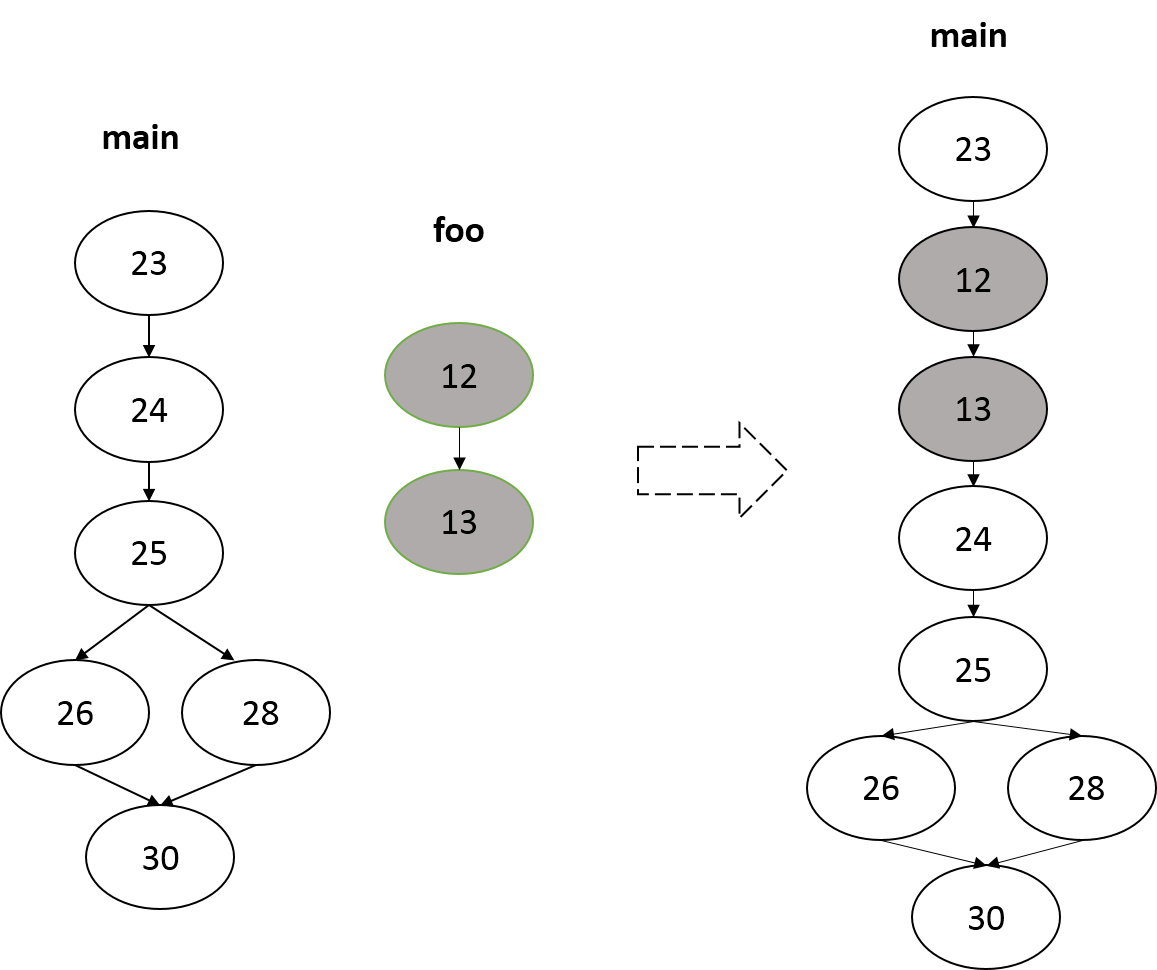
\includegraphics[width=0.70\textwidth]{figures/ICFG4-6}
	\caption{全局控制流图构建示例}\label{fig:figure4-6}
\end{figure}



\section{代码特征抽取}
分析域的全局控制流图可以表示空指针引用缺陷相关上下文代码的结构信息。但是代码不仅包含结构信息,还包含语义信息。由于本文构建的全局控制流图的结点为Jimple表示的Unit,它表示了一个抽象的语法层面的语句类型,以Unit为基本单位。基于Unit的特点,可以选取一些维度的信息进行编码作为该结点的特征附加在控制流图结构上,这些维度分别如下:

1.前驱结点数量

以构建的全局控制流图为基础,针对图中的每个结点获取其前驱结点的数量,作为该维度的特征值。

2.语句类型

Unit表示抽象的语句类型,实际上它包含了15种具体的Stmt语句类型,这些具体的语句类型和编码如表\ref{tab:table4-3}所示。

\begin{table}[hb]
	\centering
	\caption{Jimple中Stmt语句类型及特征编码} \label{tab:table4-3}
	\begin{tabular*}{0.9\textwidth}{@{\extracolsep{\fill}}ccc}
		\toprule[1pt]
		语句类别	&Stmt名称	&编码	 \\
		\midrule[1pt]
		\multirow{3}*{核心指令} &
		NopStmt	& 1	\\
		& IdentityStmt	& 2 \\
		& AssignStmt	&3 \\
		\specialrule{0em}{1pt}{1pt}
		\hline
		\specialrule{0em}{1pt}{1pt}
		
		\multirow{5}*{方法内控制流指令}	&
		IfStmt	& 4 \\
		& GotoStt	& 5 \\
		& BreakPointStmt	& 6 \\
		& TableSwitchStmt	& 7 \\
		& LookUpSwitchStmt	& 8 \\
		\specialrule{0em}{1pt}{1pt}
		\hline
		\specialrule{0em}{1pt}{1pt}
		\multirow{3}*{方法间控制流指令} &
		InvokeStmt	&9 \\
		& ReturnStmt	&10 \\
		& ReturnVoidStmt	&11 \\
		\specialrule{0em}{1pt}{1pt}
		\hline
		\specialrule{0em}{1pt}{1pt}
		\multirow{2}*{监视器指令} &
		EnterMonitorStmt	&12 \\
		& ExitMonitorStmt	&13 \\
		\specialrule{0em}{1pt}{1pt}
		\hline
		\specialrule{0em}{1pt}{1pt}
		\multirow{2}*{处理异常指令} &
		ThrowStmt	&14 \\
		& RetStmt	&15 \\
		\bottomrule[1pt]
	\end{tabular*}
\end{table}

3.调用语句类型

调用语句表明该程序涉及到了跨过程的分析,在Jimple包含的Stmt中,实现InvokeStmt接口的类有五种,它们表示五种调用方法的类型,它们的编码如表\ref{tab:table4-4}所示,如果该结点不包含方法调用语句,编码为0。

\begin{table}[hb]
	\centering
	\caption{Jimple中调用语句的类型及特征编码} \label{tab:table4-4}
	\begin{tabular*}{0.9\textwidth}{@{\extracolsep{\fill}}ccc}
		\toprule
		调用指令	&说明	&编码	 \\
		\midrule
		invokestatic & 调用静态方法	& 1	\\
		invokespecial & 调用私有方法、父类方法、构造方法	& 2 \\
		invokevirtual & 调用抽象方法	&3 \\
		invokeinterface	&调用接口方法 & 4 \\
		invokedynamic & 调用动态方法 	& 5 \\
		\bottomrule
	\end{tabular*}
\end{table}

4.使用的操作数数量

该维度特征表示了指令对操作数使用的密集程度,过多的操作数使用往往也代表着算术指令的密集使用。

5.空指针传递情况

如果当前节点涉及到了null值的传递操作,可以说明下文中有更多可能会触发空指针引用异常。空指针的传递也有不同的方式需要编码,如表\ref{tab:table4-5}所示,如果没有发生空指针传递,编码为0。

\begin{table}[ht]
	\centering
	\caption{Jimple中空指针传递类型及特征编码} \label{tab:table4-5}
	\begin{tabular*}{0.9\textwidth}{@{\extracolsep{\fill}}ccc}
		\toprule
		空指针传递指令	&传递方式	&编码	 \\
		\midrule
		ReturnStmt & 方法返回值	& 1	\\
		InvokeStmt & 方法调用传参	& 2 \\
		definitionStmt & 直接赋值	&3 \\
		\bottomrule
	\end{tabular*}
\end{table}

6.空指针检查情况

空指针检查可以很好的避免下文中对空指针的引用,该语句通常会影响到工具检测结果的判定。如果该结点对null值进行了检查,编码为1,否则为0;

通过这六个维度的特征抽取,不仅可以体现全局控制流图的结构特征,而且可以体现图中每个结点即Jimple基本语句的语义特征。但是Java代码在转换为Jimple中间表示的过程中,为了使得到的语法单位都是标准的三地址表达式,将Java基本语句进行了大量的拆解重组,使得Jimple的基本语句的粒度比Java基本语句的粒度要小很多,这就使得生成的全局控制流图所能体现的特征更加不明显。为了在模型训练的过程中更加容易的对代码分类,需要将生成的全局控制流图进一步压缩,使得图中每个结点接近基本块的维度。具体操作如算法\ref{alg:alg4-2}。

\begin{algorithm}%
	\LinesNumbered
	\KwIn{控制流图$G_c$}
	\KwOut{压缩后的控制流图$G_c'$}
	workList $\leftarrow \emptyset$  \\
	workList $\leftarrow \{G_c.RootNode\}$  \\
	\While{$worklist \neq \emptyset$}{
		node $\leftarrow$ workList.next \\
		remove node from workList \\
		node set visited \\
		\If{size of node.succList = 0}{
			node set visited \\
			continue \\
		}\ElseIf{size of node.succList = 1}{
			$tmpNode \leftarrow node$ \\
			\While{size of node.succList = 1}{
				$succNode \leftarrow node.succlist[0]$ \\
				\If{size of succNode.succList > 1 OR size of succNode.precList > 1}{
					break \\
				}
				mergeAttribute(tmpNode) \\
				$tmpNode \leftarrow succNode$ \\
				tmpNode set visited \\
			}
			$node.succList \leftarrow tmpNode.succList$ \\
			insert node into $G_c'$ \\
			\ForEach{succNode in node.succList}{
				\If{succNode is not visited}{
					insert succNode into workList \\
				}	
			}
		}\Else{
			\ForEach{succNode in node.succList}{
				\If{succNode is not visited}{
					insert succNode into workList \\
				}	
			}
		}
		insert node into $G_c'$ \\
	}
	\Return $G_c'$
	\caption{控制流图压缩算法}
	\label{alg:alg4-2}
\end{algorithm}

\begin{figure}
	\centering
	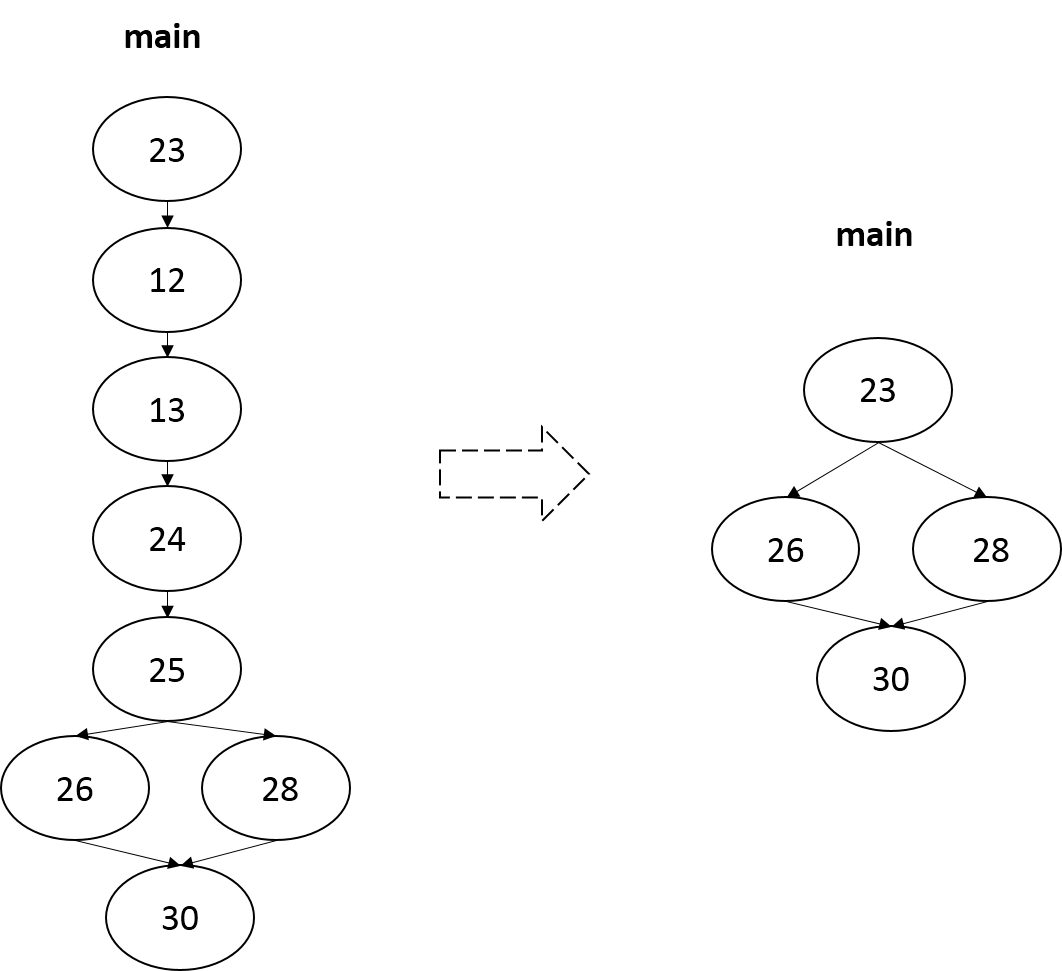
\includegraphics[width=0.70\textwidth]{figures/ICFG4-7}
	\caption{全局控制流图压缩示例}\label{fig:figure4-7}
\end{figure}


经过此算法处理,图\ref{fig:figure4-6}生成的全局控制流图将被进一步压缩,如图\ref{fig:figure4-7}所示。此算法将图中的串行结点,即前驱和后继结点数量均为1的结点合并为1个结点。同时,在算法的第16行进行了$mergeAttribute$的操作,这个操作可以将多个结点的特征属性转换到压缩后的一个结点上。具体转换方法如表\ref{tab:table4-6}所示,压缩后的图中结点的特征由压缩前多个结点的特征综合得到。

\begin{table}
	\centering
	\caption{控制流图压缩后的结点特征转换} \label{tab:table4-6}
	\begin{tabular*}{0.9\textwidth}{@{\extracolsep{\fill}}cc}
		\toprule
		压缩前特征值	&压缩后特征值	 \\
		\midrule
		前驱结点数量 & 压缩后结点的前驱结点数量	\\
		语句类型 & 被压缩结点中出现的语句类型的种类数量	 \\
		调用语句类型 & 被压缩结点中出现调用语句的数量 \\
		使用的操作数数量 & 被压缩结点中使用的操作数数量之和 \\
		调用语句类型 & 被压缩结点中调用语句的数量之和 \\
		调用语句类型 & 被压缩结点中调用语句的数量之和 \\
		\bottomrule
	\end{tabular*}
\end{table}

\section{数据标注}
前文已经提到,本文训练模型的目的是为了评估不同工具对特定缺陷检测的能力,从而根据实际结果可以预测缺陷真实的可能性。因此本文训练数据的标签应该体现工具检测相应缺陷的能力,该能力记为置信度$V(T,C,L)$,其中$T$表示工具类型,$C$表示测试用例,$L$表示测试用例中的某个具体位置,如果$V(T,C,L)=1$,表示工具$T$在用例$C$的位置$L$处的检测结果是可信的,如果$V(T,C,L)=-1$,则表示工具$T$在用例$C$的位置$L$处的检测结果不可信。

在本章第一节构建的数据集中包含两类用例,,一部分用例中包含缺陷,另一部分则为代码结构与其相似但无缺陷的用例(生成缺陷用例的原始程序)。这些用例构建完成后会添加记录缺陷位置的注解,利用注解可以构建数据集的缺陷信息库。当测试用例$C$在位置$L$处存在空指针引用缺陷时,记为$D(C,L)=1$,无缺陷时记为$D(C,L)=0$。

分别使用每种工具对目标用例进行检测,并记录测试结果。如果工具$T$在测试用例$C$的位置$L$处检测出空指针引用缺陷,记为$E(T,C,L)=1$,如果在该位置没有检测出空指针引用缺陷,则记为$E(T,C,L)=0$。然后将工具检测的结果与缺陷信息库的结果进行比对,如果工具检出的空指针引用缺陷信息与缺陷信息库中相应的缺陷信息一致,即$E(T,C,L)=D(C,L)$,则表示测试工具具备对该缺陷的检测能力,可得置信度为$V(T,C,L)=1$,否则表示测试工具不具备对该缺陷的检测能力,可得置信度$V(T,C,L)=-1$。将该置信度的值作为用例数据的标签即可。

\section{本章小结}

本章介绍了训练模型需要的数据集的来源和构造方式,以及测试用例的控制流图构建和代码特征提取的方式,此外还介绍了利用图压缩的方式来提高特征辨识度从而提升训练效率的方法。最后介绍了训练数据的标签的含义。
\chapter{深度学习模型的构建}
本章节设计了一个根据一定的分类标准分类代码的神经网络模型。模型分为两部分:图结构特征抽取模型以及特征向量分类模型。图结构特征抽取模型将代码控制流压缩为$1*d$维的向量,特征向量分类模型根据训练数据的标签对特征向量进行分类。
\par 模型以代码片段的包含节点信息的控制流图(ACFG) $g$为输入,在图结构特征抽取模型中,寻找一个合适的核函数$\phi(\cdot)$将控制流图映射到高维空间, 既能利用结点的特征信息,也保留了图结构信息。参考Hanjun Dai\cite{dai2016discriminative}等提出的方法,本文对控制流图数据用马尔可夫随机场进行建模,采用平均场推断的算法对$\phi$函数进行估计,得到了$\phi$的函数表达式。由于$\phi$函数的具体参数未知,本文采用神经网络逼近该函数,并且将特征抽取模型与分类模型连接起来,通过对训练数据的学习估计$\phi$函数。
\par 在分类模型中,本文定义了一个具有一个隐含层的神经网络,为了避免深层的网络导致过拟合的情况,采用了drop out的方法随机丢弃了一些神经元的连接。分类模型将特征抽取模型中得到的特征向量作为输入,输出一个包含工具检测正确概率以及错误概率的二维向量$[a, b]$。$a>b$时代表工具检测正确的概率较高;$a<b$代表工具检测错误的概率较高。当分类模型训练正确时,对一段陌生代码,模型应该能够正确评估不同工具对这段代码检测的结果是否正确。
\par 在训练时,将两个模型作为一个整体,随机初始化网络中的权值,运用梯度下降以及后向传播(Error BackPropagation, BP)的方法,不断更新网络中的权值,直到模型预测的检测结果与实际的检测结果相接近为止。
\label{chap:deeplearning}
\section{图结构的数据向量化}
\subsection{核函数}
\par 一般来说,对于一个给定的训练数据集$T={(x_1, y_1), (x_2, y_2), ...(x_n, y_n)}$, 其中实例$x_i$属于输入空间,$x_i\in \chi=R^n$,对应两类标签$y_i\in \gamma={-1, +1}$, 如果能用$R^n$中的一个超曲面将正负例正确的区分开,那么这个训练集则为线性不可分的。对于线性不可分的数据集,需要将原始空间映射到一个更高维的特征空间,使得数据集可以在这个特征空间里线性可分。一般来说,如果原始空间的数据维度是有限的,那么一定存在一个高维特征空间使样本可分。
\par 令$\phi(x)$表示将$x$映射过后的特征向量,那么在该特征空间下划分超平面的对应模型可以表示为:
$$f(x)=\omega^T\phi(x)+b$$
其中$w$和$b$是模型的参数。为了求出最优的划分超平面,需要求解以下最优化问题:
\begin{align}
&\min \frac{1}{2} ||\omega||^2 \\
&s.t. y_i(\omega^T\phi(x_i)+b)>=1, i=1,2,...,m.
\end{align}
对偶问题为:
\begin{align}
&\max \sum_{i=1}^{m} \alpha - \frac{1}{2}\sum_{i=1}^{m}\sum_{j=1}^{m} \alpha_i\alpha_jy_iy_j\phi(x_i)^T\phi{x_j}\\
&s.t. \sum_{i=1}^m \alpha_i y_i = 0,\\
&\phantom {s.t.}\alpha_i >=0,  i=1,2,...,m
\end{align}
\par 	求解该优化问题需要计算$\phi(x_i)^T\phi{x_j}$,该值为$x_i$和$x_j$映射到高维空间后的内积。由于高维空间的维度可能很高,甚至为无数维,因此直接计算该值是十分困难的,为了避免直接计算该值,可以定义一个核函数:
\begin{equation}
\kappa(x_i, x_j) = <\phi(x_i), \phi(x_j)> = \phi(x_i)^T\phi(x_j)
\end{equation}
即$\phi(x_i)^T\phi{x_j}$的值等于$\kappa(x_i, x_j) $,有了核函数之后,就可以避免直接计算高维甚至无穷维的内积乘法。基于此可以重写对偶问题:
\begin{align}
&\max \sum_{i=1}^{m} \alpha - \frac{1}{2}\sum_{i=1}^{m}\sum_{j=1}^{m} \alpha_i\alpha_jy_iy_j\kappa(x_i, x_j) \\
&s.t. \sum_{i=1}^m \alpha_i y_i = 0,\\
&\phantom {s.t.}\alpha_i >=0,  i=1,2,...,m
\end{align}
求解后得到分类函数:
\begin{equation}
f(x)=\sum_{i=1}^m \alpha_iy_i \kappa(x_i, x_j) +b
\end{equation}
显而易见,当已知合适的映射函数$\phi(\cdot)$的具体形式时,就可以写出核函数$\kappa(\cdot, \cdot)$的具体形式。但是在现实问题中求解合适的映射函数是十分困难的。对于图结构的数据,由于其特殊性,需要同时考虑图中结点上的语义特征以及图本身的结构特征,因此,求解其映射函数需要特殊的方法,下文将介绍图结构数据常用的核函数。
\subsection{图结构数据的核函数}
对于结构化的数据,可以通过对序列子序列的计数来构建核函数。Leslie\cite{leslie2001spectrum}等人基于此提出了谱核函数(Spectrum kernel)的概念。具体来说,对于两个结构化的数据如字符串$\chi$和$\chi'$,谱核函数定义为:
\begin{equation}
\kappa(\chi, \chi') = \sum_{s\in S}\#(s\in \chi)\#(s \in \chi')
\end{equation}
其中$S$为$\chi$和$\chi'$序列中的所有可能的子序列的集合,$\#(s\in \chi)$函数统计子序列$s$在序列$\chi$中出现的次数。相应的可以得到结构化数据的映射函数$\phi(\chi)=(\#(s_1\in \chi), \#(s_2\in \chi), ...)^T$。类似的,Sherveashidez\cite{shervashidze2009efficient}等人提出了图核函数(graphlet kernel),该函数用图结构的子图代替了谱核函数的子序列。
\par 也可以运用概率图模型的方法来构建核函数。Jaakkola和Haussler\cite{jaakkola1999using}提出了费舍尔核函数(fisher kernel),它定义了一个参数模型$p(\chi|\theta*)$, 并且通过极大似然估计的方法估计$\theta*$, 得到核函数的形式为:
\begin{equation}
\kappa(\chi, \chi') = U_\chi^TI^{-1}U_{\chi'}
\end{equation}
其中$U_\chi := \nabla_{\theta=\theta^*}\log p(\chi|\theta)$,$I=E_g[U_gU_g^T]$为费舍尔信息矩阵。
\par 为了尽可能保存图结构数据的信息,同时对图结构进行高维的转换,从而进行图结构的分类。需要找到一个映射函数$\phi$,对图结构的数据$X$,得到$\mu_x = \phi(X)$,对于合适的核函数,得到的结果$\mu$应该与$X$是等价的,也就是说对$\mu$和$X$做相同的操作,两者的结果应该相同,即:
$$f(x)=\tilde{f}(\mu_x)$$
其中$f$和$\tilde{f}$为等价的操作。在后文中将讲解如何求解$\mu_x$。
\subsection{希尔伯特空间}
希尔伯特空间将原有空间的概率分布映射到一个隐含的有限维的特征分布空间中(Smola\cite{smola2007hilbert}):
$$\mu_X = E_x [\phi(X)] = \int_X \phi(x)*p(x)dx : P\mapsto F$$
其中$P$和$F$分别为原空间与映射后的空间。这样就将求特征函数$\phi(X)$转化成了求$\phi(X)$的期望,简化了求解过程。
\section{图结构数据的建模}
\subsection{马尔可夫随机场}
马尔可夫随机场(Markov random field, MRF)是典型的马尔可夫网,是一种著名的无向图模型。图中的每个结点表示一个或一组变量,结点之间的边表示两个变量之间的依赖关系,马尔可夫随机场有一组势函数,这是定义在变量子集上的非负实函数,用于定义场中的概率分布。
\par 在马尔可夫随机场中,对于图中结点的一个子集,若其中任意两个结点都有边连接,则称该结点子集为一个“团”,若在一个团中加入另外任何一个结点都不能成“团”,则称其为“最大团”。如图\ref{fig:mrf}所示,${x_1, x_2, x_3}$不能构成“团”,${x_2, x_5}$为“团”而不是最大团。
\par 在马尔可夫随机场中,多个变量之间的联合分布能基于团分解为多个因子的乘积,每个因子仅与一个“团”有关。对于$n$个变量$x = {x_1, x_2...,x_n}$,所有团构成的集合为$C$,与团$Q\in C$对应的变量集合记为$x_Q$, 则联合概率$P(x)$定义为:
$$P(x)=\frac{1}{Z} \prod_{Q\in C} \Psi_{Q}(X_{Q})$$
其中$ \Psi_{Q}$为团$Q$对应的势函数,$Z = \sum_x \prod_{Q\in C} \Psi_{Q}(X_{Q})$为规范因子。
\begin{figure}[htbp]
	\begin{center}
		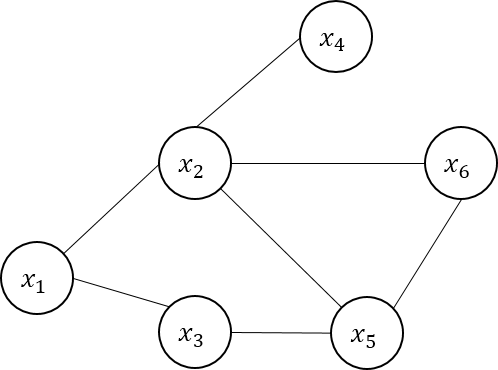
\includegraphics[width=0.5\textwidth]{figures/5-1}
		\caption{马尔可夫随机场}
		\label{fig:mrf}
	\end{center}
\end{figure}
\par 马尔可夫随机场具有两个重要的特性:
\begin{itemize}
	\item 局部马尔可夫性:给定某变量的邻接变量,则该变量条件独立于其他变量。
	\item 成对马尔可夫性:给定所有其他变量,两个非邻接变量条件独立。
\end{itemize}
\subsection{图结构数据的建模方法}
Hanjun Dai\cite{dai2016discriminative}等人用马尔可夫随机场对图结构数据进行了建模。首先定义一个图结构数据$\chi$,其结点集合为$\mathit{V}=\{1,...,V\}$,边集合为$\xi$。对图结点中的每一个结点$V_i$,都有一个对应的特征向量$X_i$。这里的特征向量$X$是能够被观测到的性质。相应的,对每一个特征向量$X_i$,可以定义一个额外的隐变量$H_i$,这样就将图结构的数据转换为了一个马尔可夫随机场,并且能够得到该随机场的联合概率分布:
\begin{equation}
p(\{H_i\}, \{X_i\}) \propto \prod_{i\in V} \Phi(H_i, X_i)\prod_{(i, j)\in \xi} \Psi(H_i, H_j)
\end{equation}
其中$\Phi$为$H_i$到$X_i$的观测函数,$\Psi$为$H_i$到$H_j$的状态转移函数。
\par 对于这个模型,在生成隐变量的过程中,不仅将图上的每个结点上的特征作为输入,还考虑到了图的结构,将新生成的隐变量的结点按图结构连接起来,从而实现了同时保留结点的属性特征和图结构特征的目的。图\ref{mod}展示了建模的过程:
\begin{figure}[htbp]
	\begin{center}
		
\includegraphics[width=0.8\textwidth]{figures//1.pdf}
		\caption{图数据隐变量建模}
		\label{mod}
	\end{center}
\end{figure}
\subsection{图结构数据模型的求解}
直接求解以上的马尔可夫随机场是十分复杂的,需要对图结构中所有结点的相互关系进行考虑,然后求解,即:
\begin{equation}
p(H_i|{x_i}) = \int_{\mathcal{H}^{V-1}} p(H_i, \{h_j\}| \{x_j\}\prod_{j\in V\i})dh_i
\end{equation}
对上式的直接求解是十分困难的,现在主要的方法是运用平均场推断和信念传播网络求解估计值,本文采用了Hanjun Dai\cite{dai2016discriminative}提出的平均场推断的算法。
\par 平均场推断算法尝试用一个独立的密度成分$q_i(h_i)$来近似估计$p(H_i|{x_i})$,即$p(H_i|{x_i})=\prod_{i\in V} q_i(h_i)$,其中$q_i(h_i)\ge 0$,在平均场中所有成分的概率和为1即$\int_\mathcal{H} q_i(h_i)dh_i=1$。求解平均场中密度成分需要最小化平均场中的自由能(Wainwright和Jordan\cite{wainwright2008graphical}),即求解以下的最优化方程:
\begin{equation}
\min_{q_1, ..., q_d} \int_\mathcal{H}^d \prod_{i\in V}q_i(h_i)\log \frac{\prod_{i\in V}q_i(h_i)}{p(\{h_i\}|\{x_i\})}\prod_{i\in V}dh_i
\end{equation}
要实现上式的最小化,需要满足以下的等式:
\begin{align}
\log q_i(h_i) &= c_i + log( \Phi(h_i, x_i)) + \sum_{j\in \mathcal{N}(i)} \int_\mathcal{H}\log (\Psi(h_i, h_j) \Phi(h_j, x_j))dh_j\\
&={c_i}'+ log( \Phi(h_i, x_i)) + \sum_{j\in \mathcal{N}(i)} \int_\mathcal{H}\log (\Psi(h_i, h_j))dh_j
\end{align}
可以得到:
$$c_i' = c_i + \sum_{j\in \mathcal{N}(i)} \int_\mathcal{H}\log \Psi(h_i, h_j)  $$
其中$\mathcal{N}(i)$为隐变量$H(i)$在图模型中的相邻结点,$c_i$为常数。从上式可以得知$q_i(h_i)$的值与$h_i, x_i, \{q_j\}_{j\in \mathcal{N}(i)}$有关,由此可以定于一个关于$q_i(h_i)$的等式:
\begin{equation}
q_i(h_i) =  f(h_i, x_i,  \{q_j\}_{j\in \mathcal{N}(i)})
\end{equation}
对于平均场中的每个组成结点$q_i$,可以得到其在希尔伯特空间的映射:
\begin{equation}
\tilde{\mu}_i = \int_{\mathcal{H}} \phi(h_i)q_i(h_i)dh_i
\end{equation}
已知$q_i(h_i) =  f(h_i, x_i,  \{q_j\}_{j\in \mathcal{N}(i)})$,可以得到:
\begin{equation}
\tilde{\mu}_i = \boldsymbol{\tau} (x_i, \{\mu_j\}_{j\in \mathcal{N}(i)})
\end{equation}
其中$\boldsymbol{\tau}$为$\tilde{\mu}_i$与$x_i, \{\mu_j\}_{j\in \mathcal{N}(i)}$的映射关系,这样不需要求解马尔可夫随机场中的$\Phi, \Psi$两个函数,就可以得到$\tilde{\mu}_i$的表示方法。对于$\boldsymbol{\tau}$函数的具体函数形式可以通过对训练数据的学习来估计。本文采用了神经网络的方法来估计该函数。
\section{分类模型的构建}
\subsection{神经网络}
神经网络是由具有适应性的简单单元组成的广泛并行互联的网络,它的组织能够模拟生物神经系统对真实世界物体所作出的交互反应\cite{kohonen1988introduction}。神经网络中最基本的成分是神经元模型,每个神经元与其他神经元互联,当它“兴奋”(接收到数据被激活)时,就会向其相邻的神经元发送数据,改变相邻神经元的值,当相邻神经元的值超过某一阈值时,该神经元就被激活,从而向其他神经元继续发送数据。
\par 1943年,McCullich 和Pitts\cite{mcculloch1943logical}将上述情形抽象为“M-P神经元模型“,结构如图\ref{fig:5-3}所示。在这个模型中,神经元接受来自n个其他神经元的信号,这些信号通过带权重的连接进行传递,神经元接受到的总输入通过激活函数处理神经元产生的输出。
\begin{figure}[htbp]
	\begin{center}
		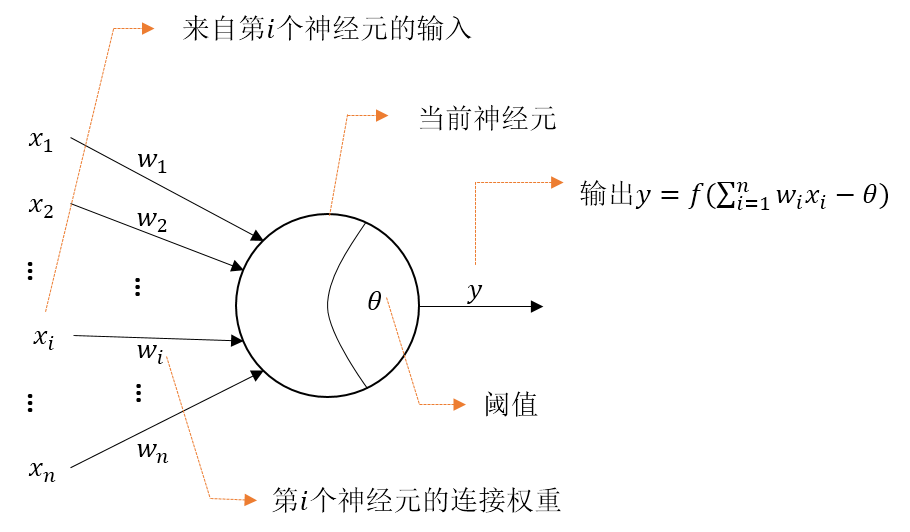
\includegraphics[width=0.75\textwidth]{figures/5-3}
		\caption{M-P神经元模型}
		\label{fig:5-3}
	\end{center}
\end{figure}
\par 图\ref{fig:5-4}展示了常用的两种激活函数。理想中的激活函数为阶跃函数,当神经元激活时,输出1,抑制时输出0。然而在实际运用中,阶跃函数具有不连续,不光滑的性质。实际常用的函数有Sigmoid函数,可以把输入压缩到(0,1)的范围内,Relu函数可以丢弃值为负的神经元。
\begin{figure}[htbp]
	\begin{center}
		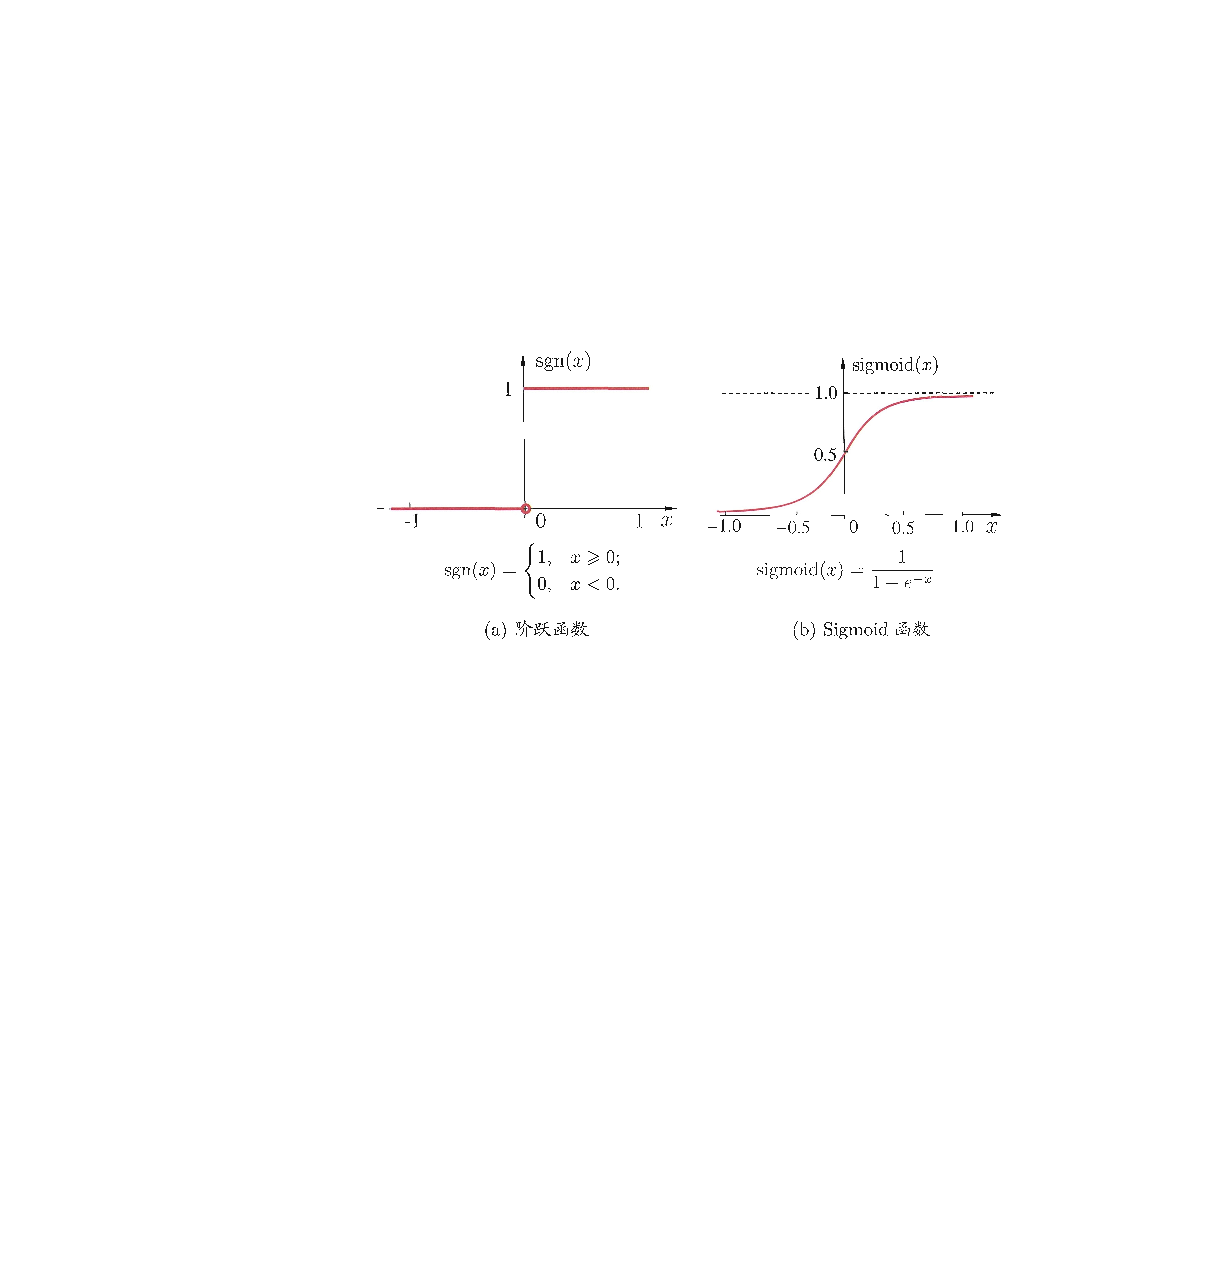
\includegraphics[width=0.8\textwidth]{figures//3.pdf}
		\caption{常用激活函数}
		\label{fig:5-4}
	\end{center}
\end{figure}
\par 从数学的角度来看,神经网络实际上是一个包含了许多参数的数学模型,可以看作是一个由$y_i = f(\sum_i w_ix_i-\theta_i)$这样的函数镶嵌叠加而成的复杂函数。当神经网络足够深时,这样的函数几乎逼近任意复杂度的连续函数,因此,可以用神经网络来代替难以求解的复杂函数,本文运用神经网络来逼近函数$\boldsymbol{\tau}$。
\subsection{图结构特征抽取模型构建}
上文中可以得到$\tilde{\mu_i}$的表示函数:
\begin{equation}
\tilde{\mu}_i = \boldsymbol{\tau} (x_i, \{\mu_j\}_{j\in \mathcal{N}(i)})
\end{equation}
先用一个一层的神经网络对该函数进行逼近,则:
\begin{equation}
\tilde{\mu}_i = \sigma(W_1x_i + W2\sum_{j\in \mathcal{N}(i)}\tilde{\mu}_j)
\end{equation}
其中$\sigma$为relu的激活函数,$W_1, W_2$为网络的权重。假设得到的隐变量$\tilde{\mu}_i$的维数为$d$,观测变量的维数为$p$,那么可以知道,$W_1$为一个$p*d$的权值矩阵,$W_2$为$d*d$的权值矩阵。为了更好的逼近函数$\boldsymbol{\tau}$,可以加深网络的深度$T$,进行多轮迭代更新$\tilde{\mu}_i$, 即:
\begin{equation}
\tilde{\mu}_i^t = \sigma(W_1x_i + W2\sum_{j\in \mathcal{N}(i)}\tilde{\mu}_j^{t-1})
\end{equation}
\begin{figure}[htbp]
	\begin{center}
		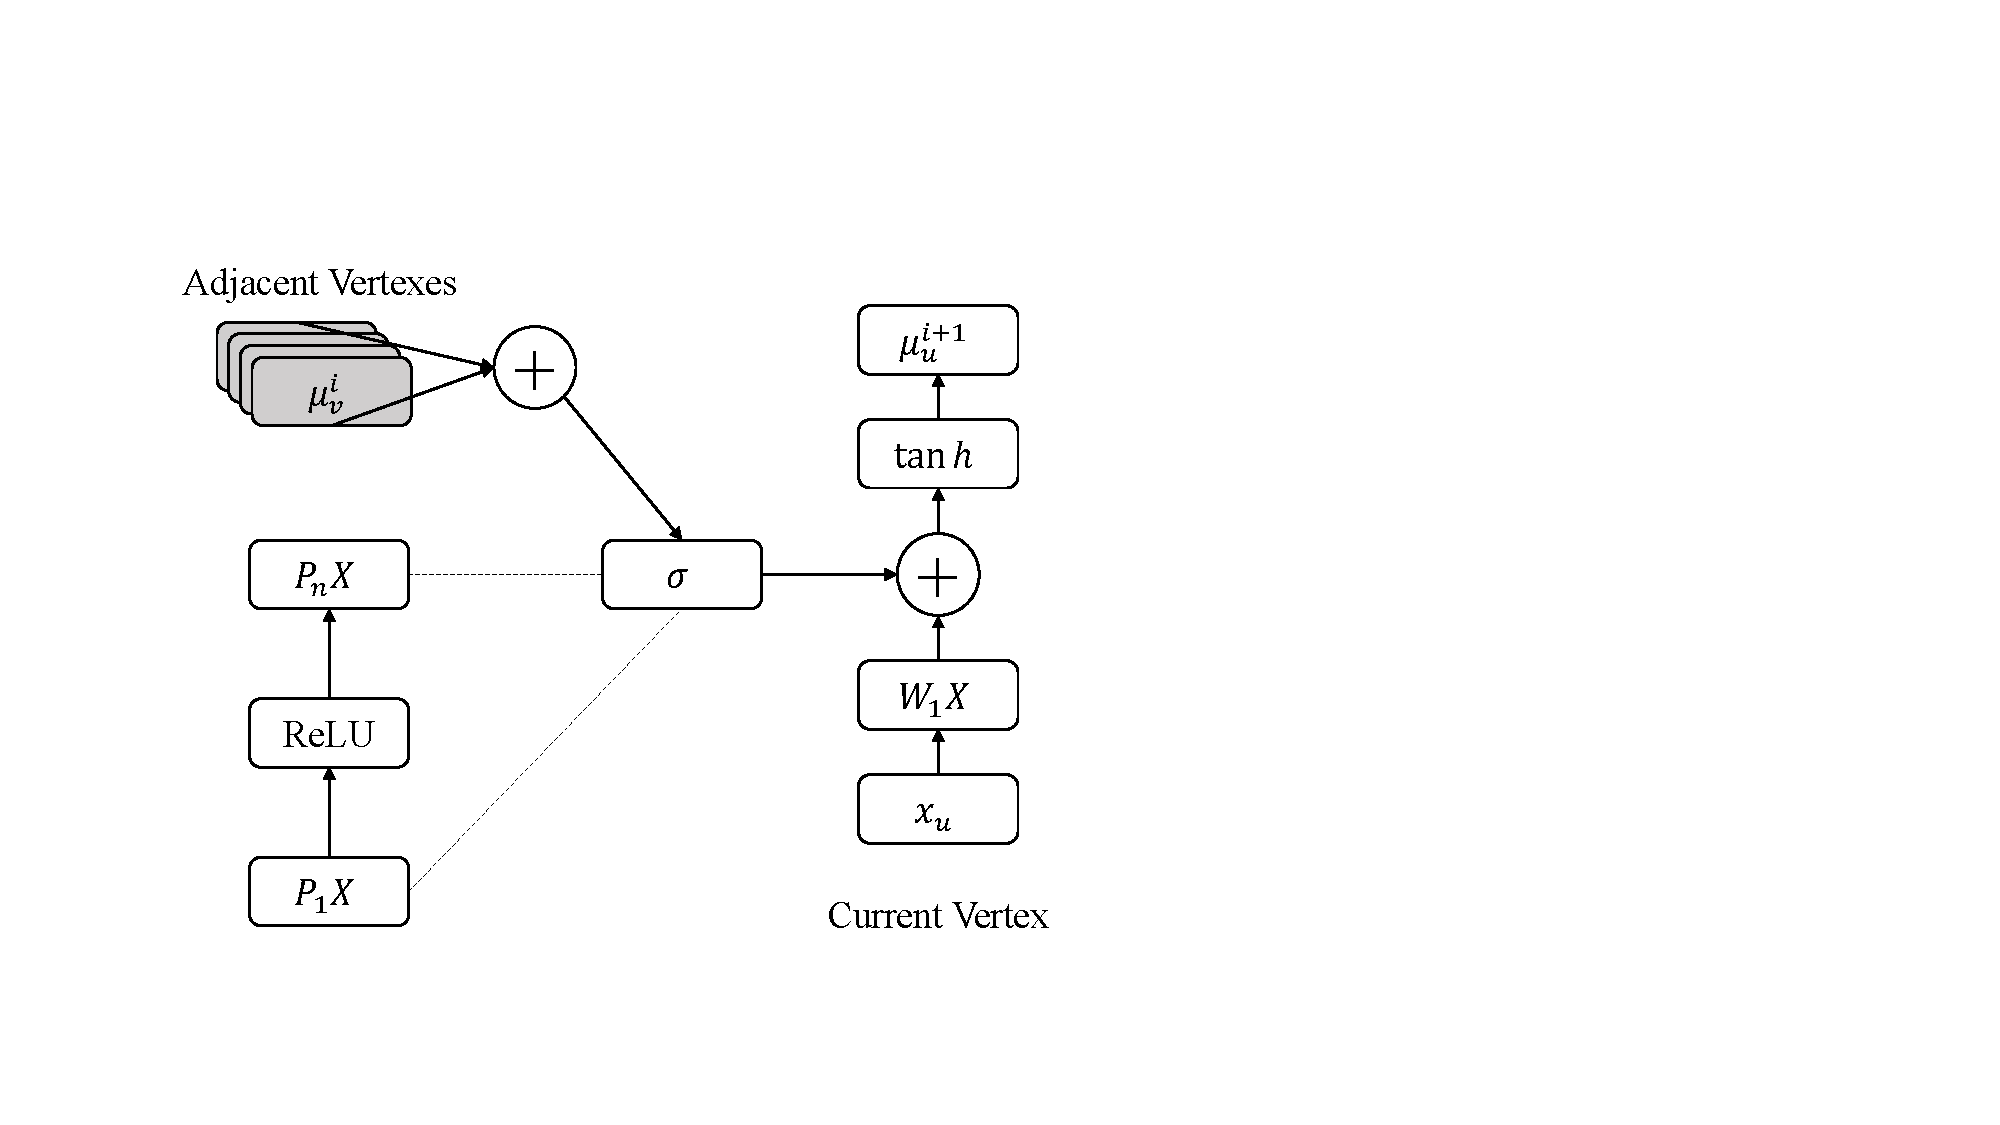
\includegraphics[width=0.7\textwidth]{figures//5.pdf}
		\caption{图特征抽取模型图示}
		\label{default}
	\end{center}
\end{figure}
至此,对图结构数据中的每一个结点,都能够得到一个隐变量$\tilde{\mu}_i$,为了将图压缩为一个$n$维的向量$g$,可以将所有结点的隐变量求和:$g =\sum_{v\in V} \mu_v^{(T)}$。$g$中包含了图结构以及图结点的信息,对$g$进行分类相当于对图结构进行分类,并且$g$作为一个n维的向量,用神经网络继续分类将十分容易。得到$g$的具体过程如算法\ref{alg:alg3}所示:
\begin{algorithm}%  
	\caption{Graph embedding algorithm}  
	\KwIn{$ACFG g = (V, \xi, x)$}
	\KwOut {$\phi(g)$}
	Initialize $\mu_v^{(0)} = \overline{0}$, for all $v \in V$\\
	\For {$t = 1 \KwTo T$}{
		\ForEach{$v\in V$}{
			$l_v = \sum_{u\in \mathcal{N}(v)}\mu_{u}^{(t-1)}$\\
			$\mu_v^{(t)} = tanh(W_1*x_v+\sigma(W_2*l_v)$\\
		}
	}
	\Return {$\phi(g) = \sum_{v\in V} \mu_v^{(T)}$}
	\label{alg:alg3}
\end{algorithm}
  
\subsection{判别模型的构建}
明确了图数据压缩网络后,就可以通过训练数据来学习网络中的参数。为了判定某段代码能否被一个静态检测工具正确的检测,需要一些先验的数据集 $D={x_n, y_n}_{n=1}^N$,其中$x_n$为抽取出来的代码的控制流图,$y_n$为代码的标签。如果该代码能够被工具正确检测,$y_n=[1, 0]$,否则$y_n=[0, 1]$,这是一个二分类的问题。需要学习得到一个网络,使网络得到的值能够最大的拟合训练数据,即:
\begin{align}
&\min \sum_{n=1}^{N} (y_n - P*\phi(g))\\
&=\min \sum_{n=1}^{N} y_n - P*(\sum_{i=1}^{V_n} \tilde{\mu}_i^n)
\end{align}
为了更好的拟合数据集$D$,逼近真实函数,本文在图结构压缩网络上定义了一个两层的非全连接网络$P$, $P$在两层全连接网络的基础上随机丢弃了一些神经元,从而避免了全连接网络可能存在的过拟合问题,具体来说,$P$可以定义为:
\begin{equation}
P(\phi(g)) = W_4*(relu(W_3*relu(\phi(g))))
\end{equation}
其中$W_3$为$d*d$的权值矩阵,$W_4$为$d*2$的权值矩阵。这样就得到了一个完整的图结构数据分类网络,该网络有四个权值矩阵$W_1, W_2, W_3, W_4$,以代码的控制流图为输入,输出一个$1*2$的向量$[a, b]$。当输出$a>b$时,代表工具检测正确的可能性大于错误的可能性;若$a<b$代表工具检测错误的可能性更大。本文用梯度下降的方法对网络的权值进行更新,当输出值$[a, b]$与训练集的标签$y_n$残差较小且趋于稳定时,就得到了一个较好的用于区分某段代码能否被工具正确检测的分类网络。
\begin{figure}[htbp]
	\begin{center}
		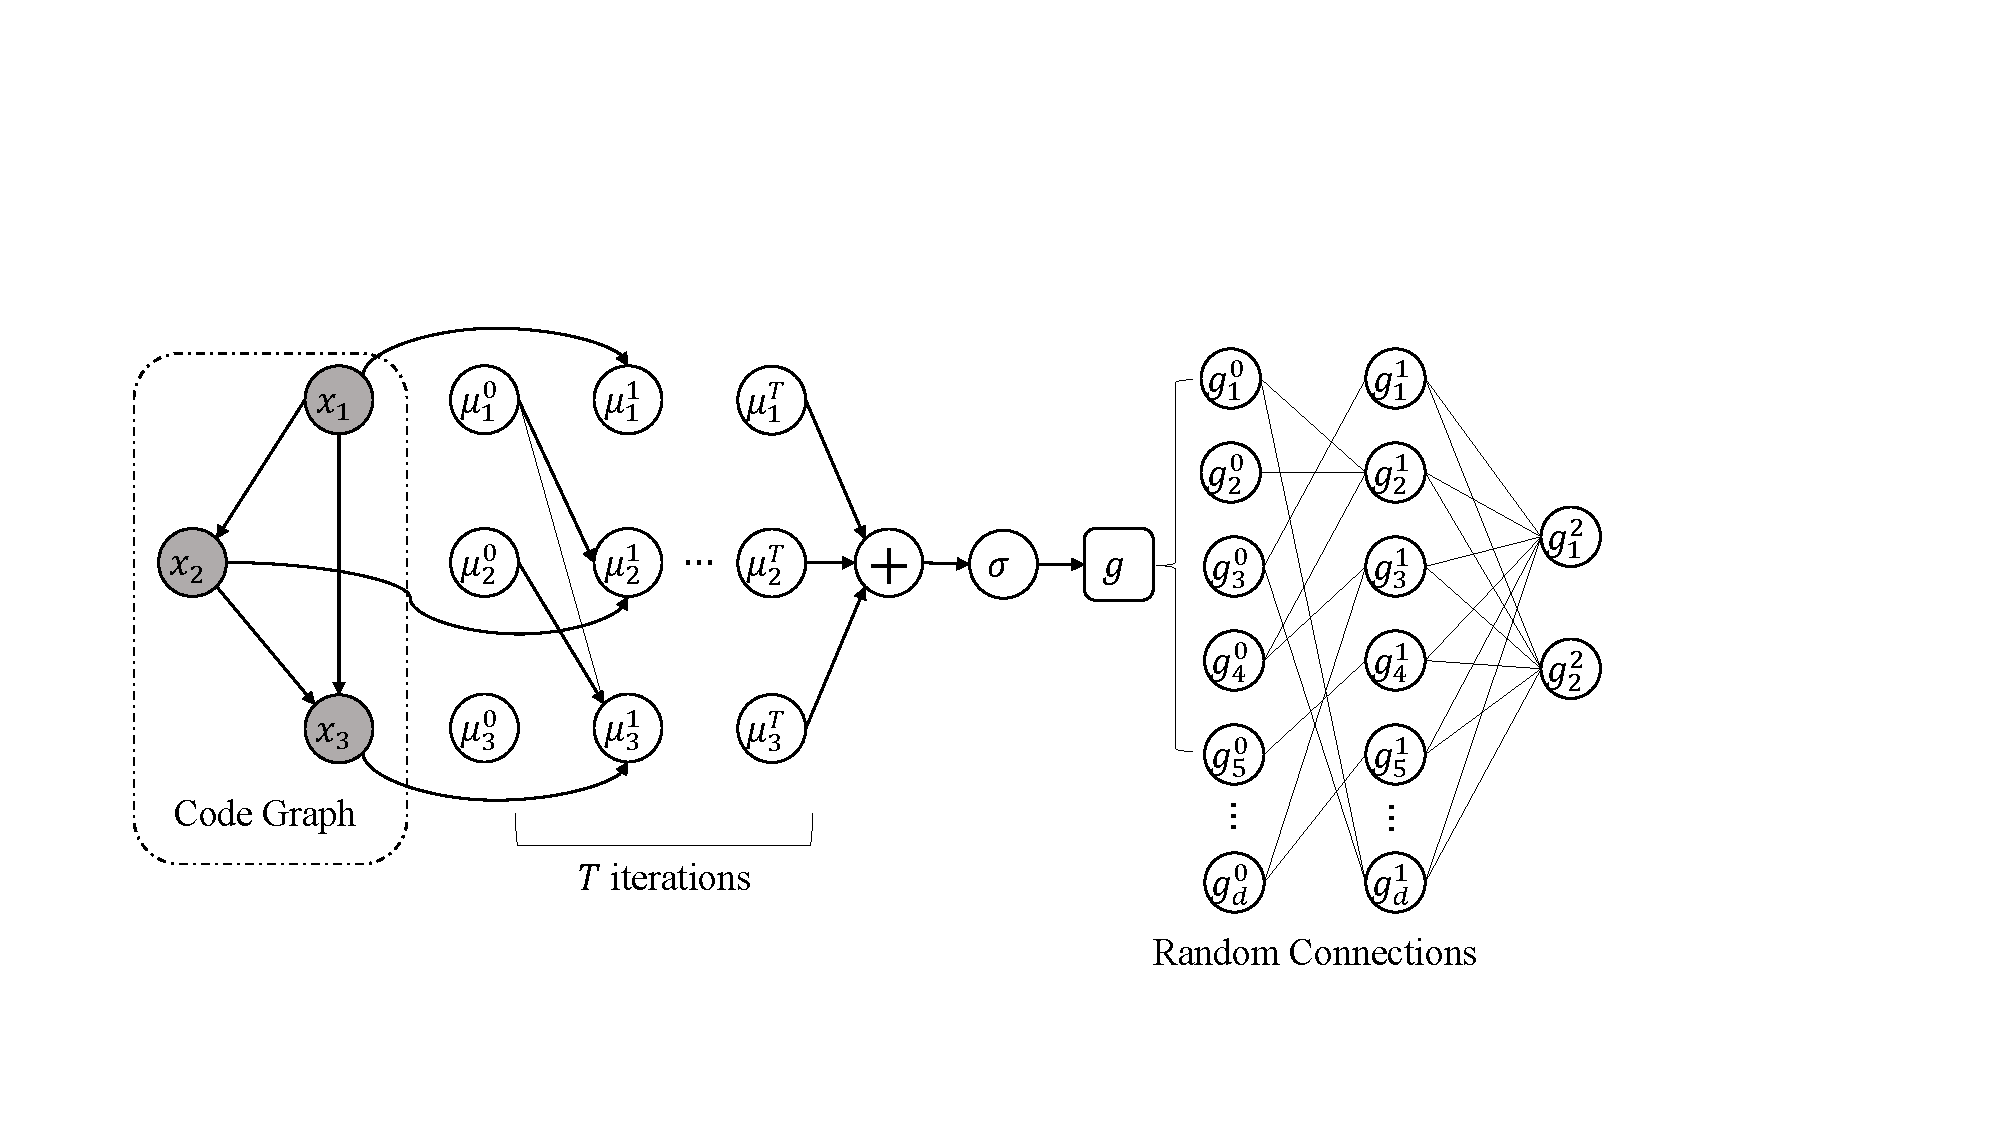
\includegraphics[width=0.95\textwidth]{figures//6.pdf}
		\caption{完整分类模型图示}
		\label{default}
	\end{center}
\end{figure}
\par 基于此,对于四个静态代码分析工具,最终能训练出四个相应的分类器,这样,当检测目标代码时,四个分类器能够分别得到四个工具检测这段代码的置信度$W = \{w_1, w_2, w_3, w_4\}$,同时还能够得到四个工具对这段代码的检测结果$R = \{r_1, r_2, r_3, r_4\}$,综合两个结果,就能够得到这段代码是否真正出现了空指针引用缺陷:
$$P = W^T*R = \sum_{i=1}^4 w_i*r_i$$
\par 设定好一个阈值$p$,当$P\le p$时,推断该代码段存在空指针引用缺陷;$P>p$,推断该代码不存在空指针引用缺陷。阈值$p$也可以通过学习得到,通过试错的方法逐渐更新$p$值,直到在训练集和测试集上得到最高的测试准确率时,停止更新。
\section{本章小结}
本章介绍了代码分类神经网络模型的基本构造,阐述了图数据特征抽取模型的理论基础以及设计原理,介绍了分类模型神经网络的连接方式。最后阐明了神经网络的训练方法以及评判标准。
%%==================================================
%% conclusion.tex for BIT Master Thesis
%% modified by yang yating
%% version: 0.1
%% last update: Dec 25th, 2016
%%==================================================


\begin{conclusion}

随着大数据时代的到来,信息技术与互联网的快速发展,数据量呈爆炸式增长。数据中包含着巨大的价值,而如何从海量的数据中挖掘出对人类有价值的信息,是现代社会的一个巨大的挑战与机遇。数据的压缩与异常数据检测,是在数据的分析与挖掘模型中重要的两个环节,在工业与生活中,也具有广泛的应用。流式数据是大数据中重要的一种形式。在对流式数据的处理与分析中,存在着以下几个问题。首先,是数据的存储问题,流式数据的数据量巨大,已有的存储介质不能存储所有的原始数据,所以,一些适用于静态数据集的挖掘方法无法直接使用在流式数据上。然后,是计算的实时性问题,流式数据是快速而且持续地产生的,计算的实时性尤其重要,如果数据处理不及时,很有可能发生数据的堆积,从而造成数据丢失。最后,流式数据往往是动态变化的,数据的分布总在变化,这使得很多静态数据集上研究的算法无法适应,效率与性能大大降低。上述的这些问题,给流式数据的研究带来了困难与挑战。基于上述问题,本文主要对流式数据的数据压缩与异常数据检测的加速进行了研究,使其能够快速计算,保证流式数据处理的实时性。本文的主要研究成果可以概括如下:

一,对数据的异常数据检测与数据的压缩进行了研究与总结。总结介绍了异常数据的定义,异常数据是不符合正常行为模式定义的数据模式,异常数据分为点异常,上下文异常和集体异常。而且异常数据检测的输出有分数型和标记型两种形式。然后又介绍了异常数据检测的相关算法,分析了各种算法的优缺点与使用范围。介绍了数据压缩的意义和现有的数据压缩算法,包括分段表示法、频域法、奇异值分解法与符号表示法。分析了各种算法的优缺点与使用范围,并且阐述了分段表示法最常使用的原因。

二,在对流式数据进行异常数据检测时,针对流式数据数据量巨大的特点,提出了改进的增量LOF算法。第一,将其空间划分为多个网格,将流式数据的数据点映射到网格中,可以解决流式数据数据量大,无法全部存储的问题。第二,设计网格的特征向量,将网格中的有权值的中心点代替映射到网格中的所有数据点,来进行增量的LOF算法的检测,可以减少计算量,加速检测异常数据速度,保证流式计算的实时性。第三,实验表明,该算法不但可以有效检测出异常数据,而且检测异常数据的速度更快,效率更高。

三,在对流式数据进行压缩时,选择简单直观常用的分段多项式拟合算法,提出了加速算法。第一,针对分段多项式拟合,给出了最小二乘法的解决过程。第二,针对静态时序数据的压缩,分别给出了平均分段与不平均分段的加速方法,通过建立缓存,来直接使用之前的计算结果,减少矩阵计算,加快了计算的速度。并且分别针对周期时间采集的与非周期时间采集的时序数据,给出了不同的加速方式。第三,针对流式时序数据,给出了使用滑动窗口算法的压缩过程,而且对于周期时间采样的时序数据,根据其时刻序号的特点,给出了使用缓存减少计算量的方法,加速压缩过程。针对非周期时间采样的时序数据,因为采样间隔不确定,所以不再使用空间替换时间的方法,而提出一种增量计算的方法,减少计算量和窗口内的数据点的存储量,提高了计算效率。

\end{conclusion}

%% 参考文献,五号字,使用 BibTeX,包含参考文献文件.bib

%\bibliography{reference/chap1,reference/chap2} %多个章节的参考文献
\bibliography{reference/luohui}


%%%%%%%%%%%%%%%%%%%%%%%%%%%%%%
%% 后置部分
%%%%%%%%%%%%%%%%%%%%%%%%%%%%%%

%% 附录(章节编号重新计算,使用字母进行编号)
\appendix
\renewcommand\theequation{\Alph{chapter}--\arabic{equation}}  % 附录中编号形式是"A-1"的样子
\renewcommand\thefigure{\Alph{chapter}--\arabic{figure}}
\renewcommand\thetable{\Alph{chapter}--\arabic{table}}

%%%==================================================
%% app1.tex for BIT Master Thesis
%% modified by yang yating
%% version: 0.1
%% last update: Dec 25th, 2016
%%==================================================


\chapter{***}

附录相关内容…
 
%
\chapter{Maxwell Equations}


因为在柱坐标系下,$\overline{\overline\mu}$是对角的,所以Maxwell方程组中电场$\bf
E$的旋度

所以$\bf H$的各个分量可以写为:
\begin{subequations}
  \begin{eqnarray}
    H_r=\frac{1}{\mathbf{i}\omega\mu_r}\frac{1}{r}\frac{\partial
      E_z}{\partial\theta } \\
    H_\theta=-\frac{1}{\mathbf{i}\omega\mu_\theta}\frac{\partial E_z}{\partial r}
  \end{eqnarray}
\end{subequations}
同样地,在柱坐标系下,$\overline{\overline\epsilon}$是对角的,所以Maxwell方程组中磁场$\bf
H$的旋度
\begin{subequations}
  \begin{eqnarray}
    &&\nabla\times{\bf H}=-\mathbf{i}\omega{\bf D}\\
    &&\left[\frac{1}{r}\frac{\partial}{\partial
        r}(rH_\theta)-\frac{1}{r}\frac{\partial
        H_r}{\partial\theta}\right]{\hat{\bf
        z}}=-\mathbf{i}\omega{\overline{\overline\epsilon}}{\bf
      E}=-\mathbf{i}\omega\epsilon_zE_z{\hat{\bf z}} \\
    &&\frac{1}{r}\frac{\partial}{\partial
      r}(rH_\theta)-\frac{1}{r}\frac{\partial
      H_r}{\partial\theta}=-\mathbf{i}\omega\epsilon_zE_z
  \end{eqnarray}
\end{subequations}
由此我们可以得到关于$E_z$的波函数方程:
\begin{eqnarray}
  \frac{1}{\mu_\theta\epsilon_z}\frac{1}{r}\frac{\partial}{\partial r}
  \left(r\frac{\partial E_z}{\partial r}\right)+
  \frac{1}{\mu_r\epsilon_z}\frac{1}{r^2}\frac{\partial^2E_z}{\partial\theta^2}
  +\omega^2 E_z=0
\end{eqnarray}
 

%(其后部分无编号)
\backmatter

% 发表文章目录
%%==================================================
%% pub.tex for BIT Master Thesis
%% modified by yang yating
%% version: 0.1
%% last update: Dec 25th, 2016
%%==================================================

\begin{publications}{99}

    \item\textsc{高凌}. {交联型与线形水性聚氨酯的形状记忆性能比较}[J].
      化工进展, 2006, 532-535.(核心期刊)
    
\end{publications}

% 致谢
%%==================================================
%% thanks.tex for BIT Master Thesis
%% modified by yang yating
%% version: 0.1
%% last update: Dec 25th, 2016
%%==================================================

\begin{thanks}
行文至此,我的硕士生涯也就像这篇毕业论文一样走到了尾声。

在北理的两年生活,虽然还是习惯了实验室,食堂和宿舍的三点一线,但是已经感觉到自己从适应学校到适应社会的转变。参加了一些学术会议,见识了很多大牛,慢慢懂得了对待学术应该更加谦卑。参加了一些社会实践,感受了职场生活,也慢慢懂得了对待工作应该更加专业。更重要的,慢慢懂得了应试能力和学习能力的区别,明白了生活是一道主观题而不是客观题,学会了去承担责任,做出取舍。

面对不断逼近的六月,离别也如期而至。解锁人生新关卡带来的激动和喜悦很快便被不舍和失落淹没。在跟过去道别之前,首先要感谢我的导师田东海老师和计卫星老师,他们在本论文的选题和研究上给予了重要的帮助。学贵得师,亦贵得友,两位老师谦和严谨而又不失活泼的处事风格无论在学术上还是生活上都深深地感染着我,能够遇到两位老师是我这两年来的最大幸事。

然后感谢实验室的小伙伴:杨恬,高建花,谈兆年,张莎莎,他们对本文的顺利完成也提供了必要的帮助。还有其他在实验室一路陪伴我的兄弟姐妹:石剑君,田泽民,李安民,以及已经毕业的郑兴生,付文飞,高志伟,廖心怡,张露露,张晶晶。我会记得永远充满欢声笑语的931,一起讨论问题抑或欣赏电影的930,一起挥洒过汗水的羽毛球场,一起品尝过的美味大餐,以及所有一起爬过的山,走过的路。

特别感谢我的父母,感谢他们在背后默默的支持,平凡而伟大的亲情永远是我无畏前行的后盾!

还要感谢离我而去的人,是你让我懂得了怎么去爱和珍惜!

最后替十年后的我感谢现在一直努力的自己!

所有BIT的朋友,山高水长,江湖再见!








\end{thanks}

% 作者简介(博士论文需要)
%%%==================================================
%% resume.tex for BIT Master Thesis
%% modified by yang yating
%% version: 0.1
%% last update: Dec 25th, 2016
%%==================================================

\begin{resume}

本人…。

\end{resume}



\end{document}
